\documentclass[12pt,aspectratio=169]{beamer}

\usetheme[progressbar=frametitle]{metropolis}
\usepackage{appendixnumberbeamer}

\usepackage{booktabs}
\usepackage[scale=2]{ccicons}

\usepackage{pgfplots}
\usepgfplotslibrary{dateplot}

\usepackage{xspace}
\newcommand{\themename}{\textbf{\textsc{metropolis}}\xspace}

\usepackage{datetime}

\usepackage{threeparttable}
\usepackage{multirow}
\usepackage{tabularx}
\usepackage[]{siunitx}
\usepackage{makecell}
\usepackage{diagbox}
\usepackage[absolute,overlay]{textpos}
\usepackage{etoolbox}
\usepackage{microtype}
\usepackage{tcolorbox}
\usepackage[author={Micha\"{e}l Roynard}]{pdfcomment}
%\usepackage{setspace}

\usepackage{pdfpcnotes}

% Grid
%\usepackage[texcoord,grid,gridunit=mm,gridcolor=red!10,subgridcolor=green!10]{eso-pic}


\usepackage{pifont}
\newcommand{\cmark}{\textcolor{green!50!white}{\ding{51}}}%
\newcommand{\xmark}{\textcolor{red!50!white}{\ding{55}}}%
\newcommand{\eqmark}{{\bf \(\approx\)}}

\definecolor{lightgray}{rgb}{0.68, 0.68, 0.68}
\definecolor{lightblue}{rgb}{0.68, 0.85, 0.9}
\definecolor{lightgreen}{rgb}{0.56, 0.93, 0.56}
\definecolor{thistle}{rgb}{0.85, 0.75, 0.85}

\newcommand{\GRAYOUT}[1]{\textcolor{lightgray}{#1}}%

\setbeamerfont{subsection in toc}{size=\scriptsize}

%\makeatletter
%\patchcmd{\beamer@sectionintoc}{\vskip1.5em}{\vskip0.5em}{}{}
%\makeatother

\usepackage{soul}
%\sethlcolor{yellow!60!white}

\makeatletter
\let\HL\hl
\renewcommand\hl{%
  \let\set@color\beamerorig@set@color
  \let\reset@color\beamerorig@reset@color
  \HL}
\makeatother

\usepackage{minted}
\setminted{fontsize=\scriptsize}

\newdate{dateSoutenance}{04}{11}{2022}

\usepackage{bibentry}
\usepackage[backend=biber,
          bibencoding=utf8,
            defernumbers=true,
            sorting=ynt,
            %style=numeric,
            style=apa,
            %style=apa,
            %style=draft,
            backref=true]{biblatex}
\addbibresource{../bibliography.bib}

\usepackage{xpatch}
% shorten author
%\xapptobibmacro{cite}{\setunit{\nametitledelim}\printfield{booktitle}}{}{}

\title{Generic programming in modern C++ for\\ Image Processing}
%\subtitle{}
\date{Thesis Defense --- \displaydate{dateSoutenance}}
\author{\textbf{Michaël Roynard} \hspace{1cm} Director: \emph{Thierry Géraud} \hspace{1cm} Supervisor: \emph{Edwin Carlinet}}
\institute{EPITA Research Laboratory (LRE) --- Le Kremlin-Bicêtre, France}
\titlegraphic{

\includegraphics[width=.2\textwidth]{../images/logo-edite}\hfill

\includegraphics[width=.2\textwidth]{../images/epita}\hfill

\includegraphics[width=.2\textwidth]{../images/lre-logo.png}\hfill

\includegraphics[width=.2\textwidth]{../images/Logo_of_Sorbonne_University}
}

\makeatletter
\setbeamertemplate{title page}{
  \begin{minipage}[b][\paperheight]{\textwidth}
    \vfill%
    \ifx\inserttitle\@empty\else\usebeamertemplate*{title}\fi
    \ifx\insertsubtitle\@empty\else\usebeamertemplate*{subtitle}\fi
    \usebeamertemplate*{title separator}
    \ifx\beamer@shortauthor\@empty\else\usebeamertemplate*{author}\fi
    \ifx\insertdate\@empty\else\usebeamertemplate*{date}\fi
    \ifx\insertinstitute\@empty\else\usebeamertemplate*{institute}\fi
    \vfill
    \ifx\inserttitlegraphic\@empty\else\inserttitlegraphic\fi
    \vspace*{1cm}
  \end{minipage}
}
\makeatother

% diapo accorche
% diapo 16
% enchainement 29-30
% 32, 34, 38, 48
% transition conclusion

\begin{document}

\maketitle

\begin{frame}{Overview}
  \setbeamertemplate{section in toc}[sections numbered]
  %\singlespacing
  \tableofcontents[hideallsubsections]
  \pdfcomment[icon=Note]{Introduction -> Domaine du traitement d'image et justifier le besoin en généricité}
  \pdfcomment[icon=Note]{   }
  \pdfcomment[icon=Note]{Context \& History -> Comment on passe d'un algorithme non-générique à un algorithme générique}
  \pdfcomment[icon=Note]{Généricité non contrainte à généricité contrainte}
  \pdfcomment[icon=Note]{   }
  \pdfcomment[icon=Note]{Programmation générique pour le traitement d'image -> 1ère contribution un environnement pour faire de
    la généricité contraintes pour le traitement d'image dans un monde statique (compilation)}
  \pdfcomment[icon=Note]{   }
  \pdfcomment[icon=Note]{Vues pour le traitement d'image -> 2nd contribution -> Design d'un nouveau niveau d'abstration
    (utilisant le 1er environnement) : les Vues -> ce sont des types d'images embarquant des algorithmes}
  \pdfcomment[icon=Note]{   }
  \pdfcomment[icon=Note]{Conclusion \& perspectives -> nous conclurons sur notre travail et discuterons des pistes à explorer à l'avenir}
  \pnote{
    Introduction -> Domaine du traitement d'image et justifier le besoin en généricité

    Context & History -> Comment on passe d'un algorithme non-générique à un algorithme générique
    Généricité non contrainte à généricité contrainte

    Programmation générique pour le traitement d'image -> 1ère contribution
    un environnement pour faire de la généricité contraintes pour le traitement d'image dans un monde statique (compilation)

    Vues pour le traitement d'image -> 2nd contribution
    design d'un nouveau niveau d'abstraction (utilisant le 1er environnement) : les vues
    ce sont des types d'images embarquant des algorithmes

    Conclusion & perspectives -> nous conclurons sur notre travail et discuterons des pistes à explorer à l'avenir
  }
\end{frame}

%
%
%

\section[Introduction]{Introduction}

\begin{frame}[fragile]{Image processing nowadays}
  \begin{itemize}
    \item Every industry and research domain is using it \GRAYOUT{(production line automation, automatic document
            reading, social network apps, etc.)}
    \item Image processing is everywhere, in most of the devices \GRAYOUT{(computer, phone, embedded devices, etc.)}
    \item Applications are multiples \GRAYOUT{(medical imaging, social network filters, facial recognition, etc.)}
    \item Image Processing is costly in resources. Performance is crucial.
  \end{itemize}
  \begin{figure}[bl]
    \hfill
    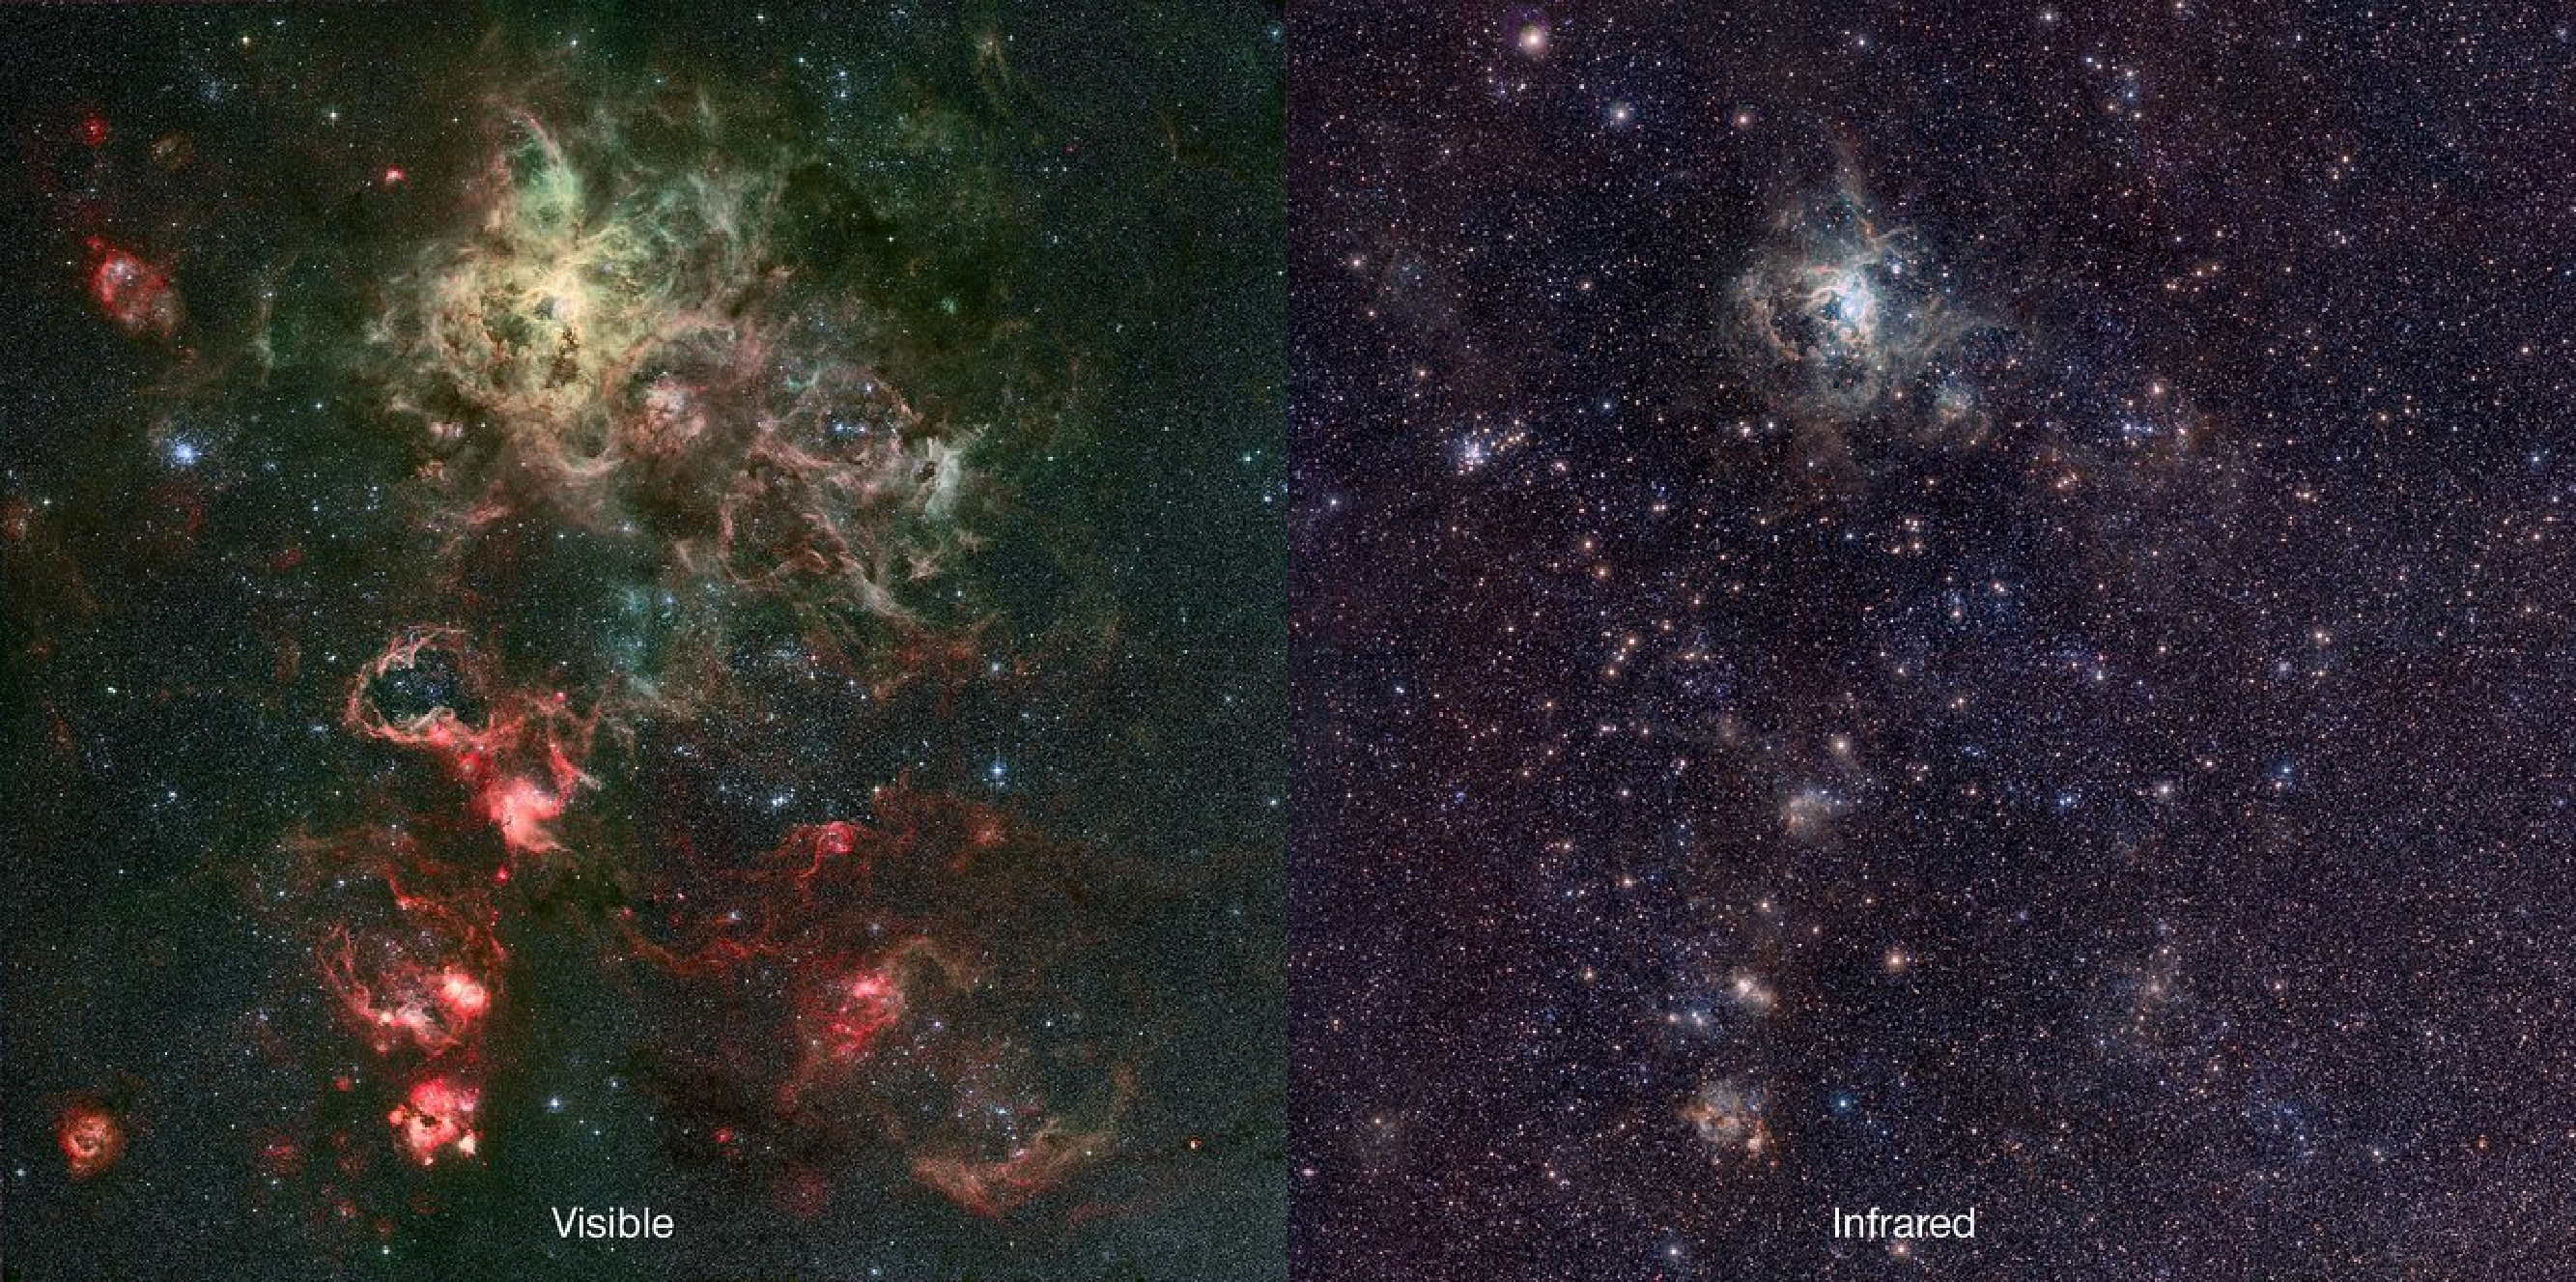
\includegraphics[height=3cm]{../illustrations/rgb_infrared}
    \hfill
    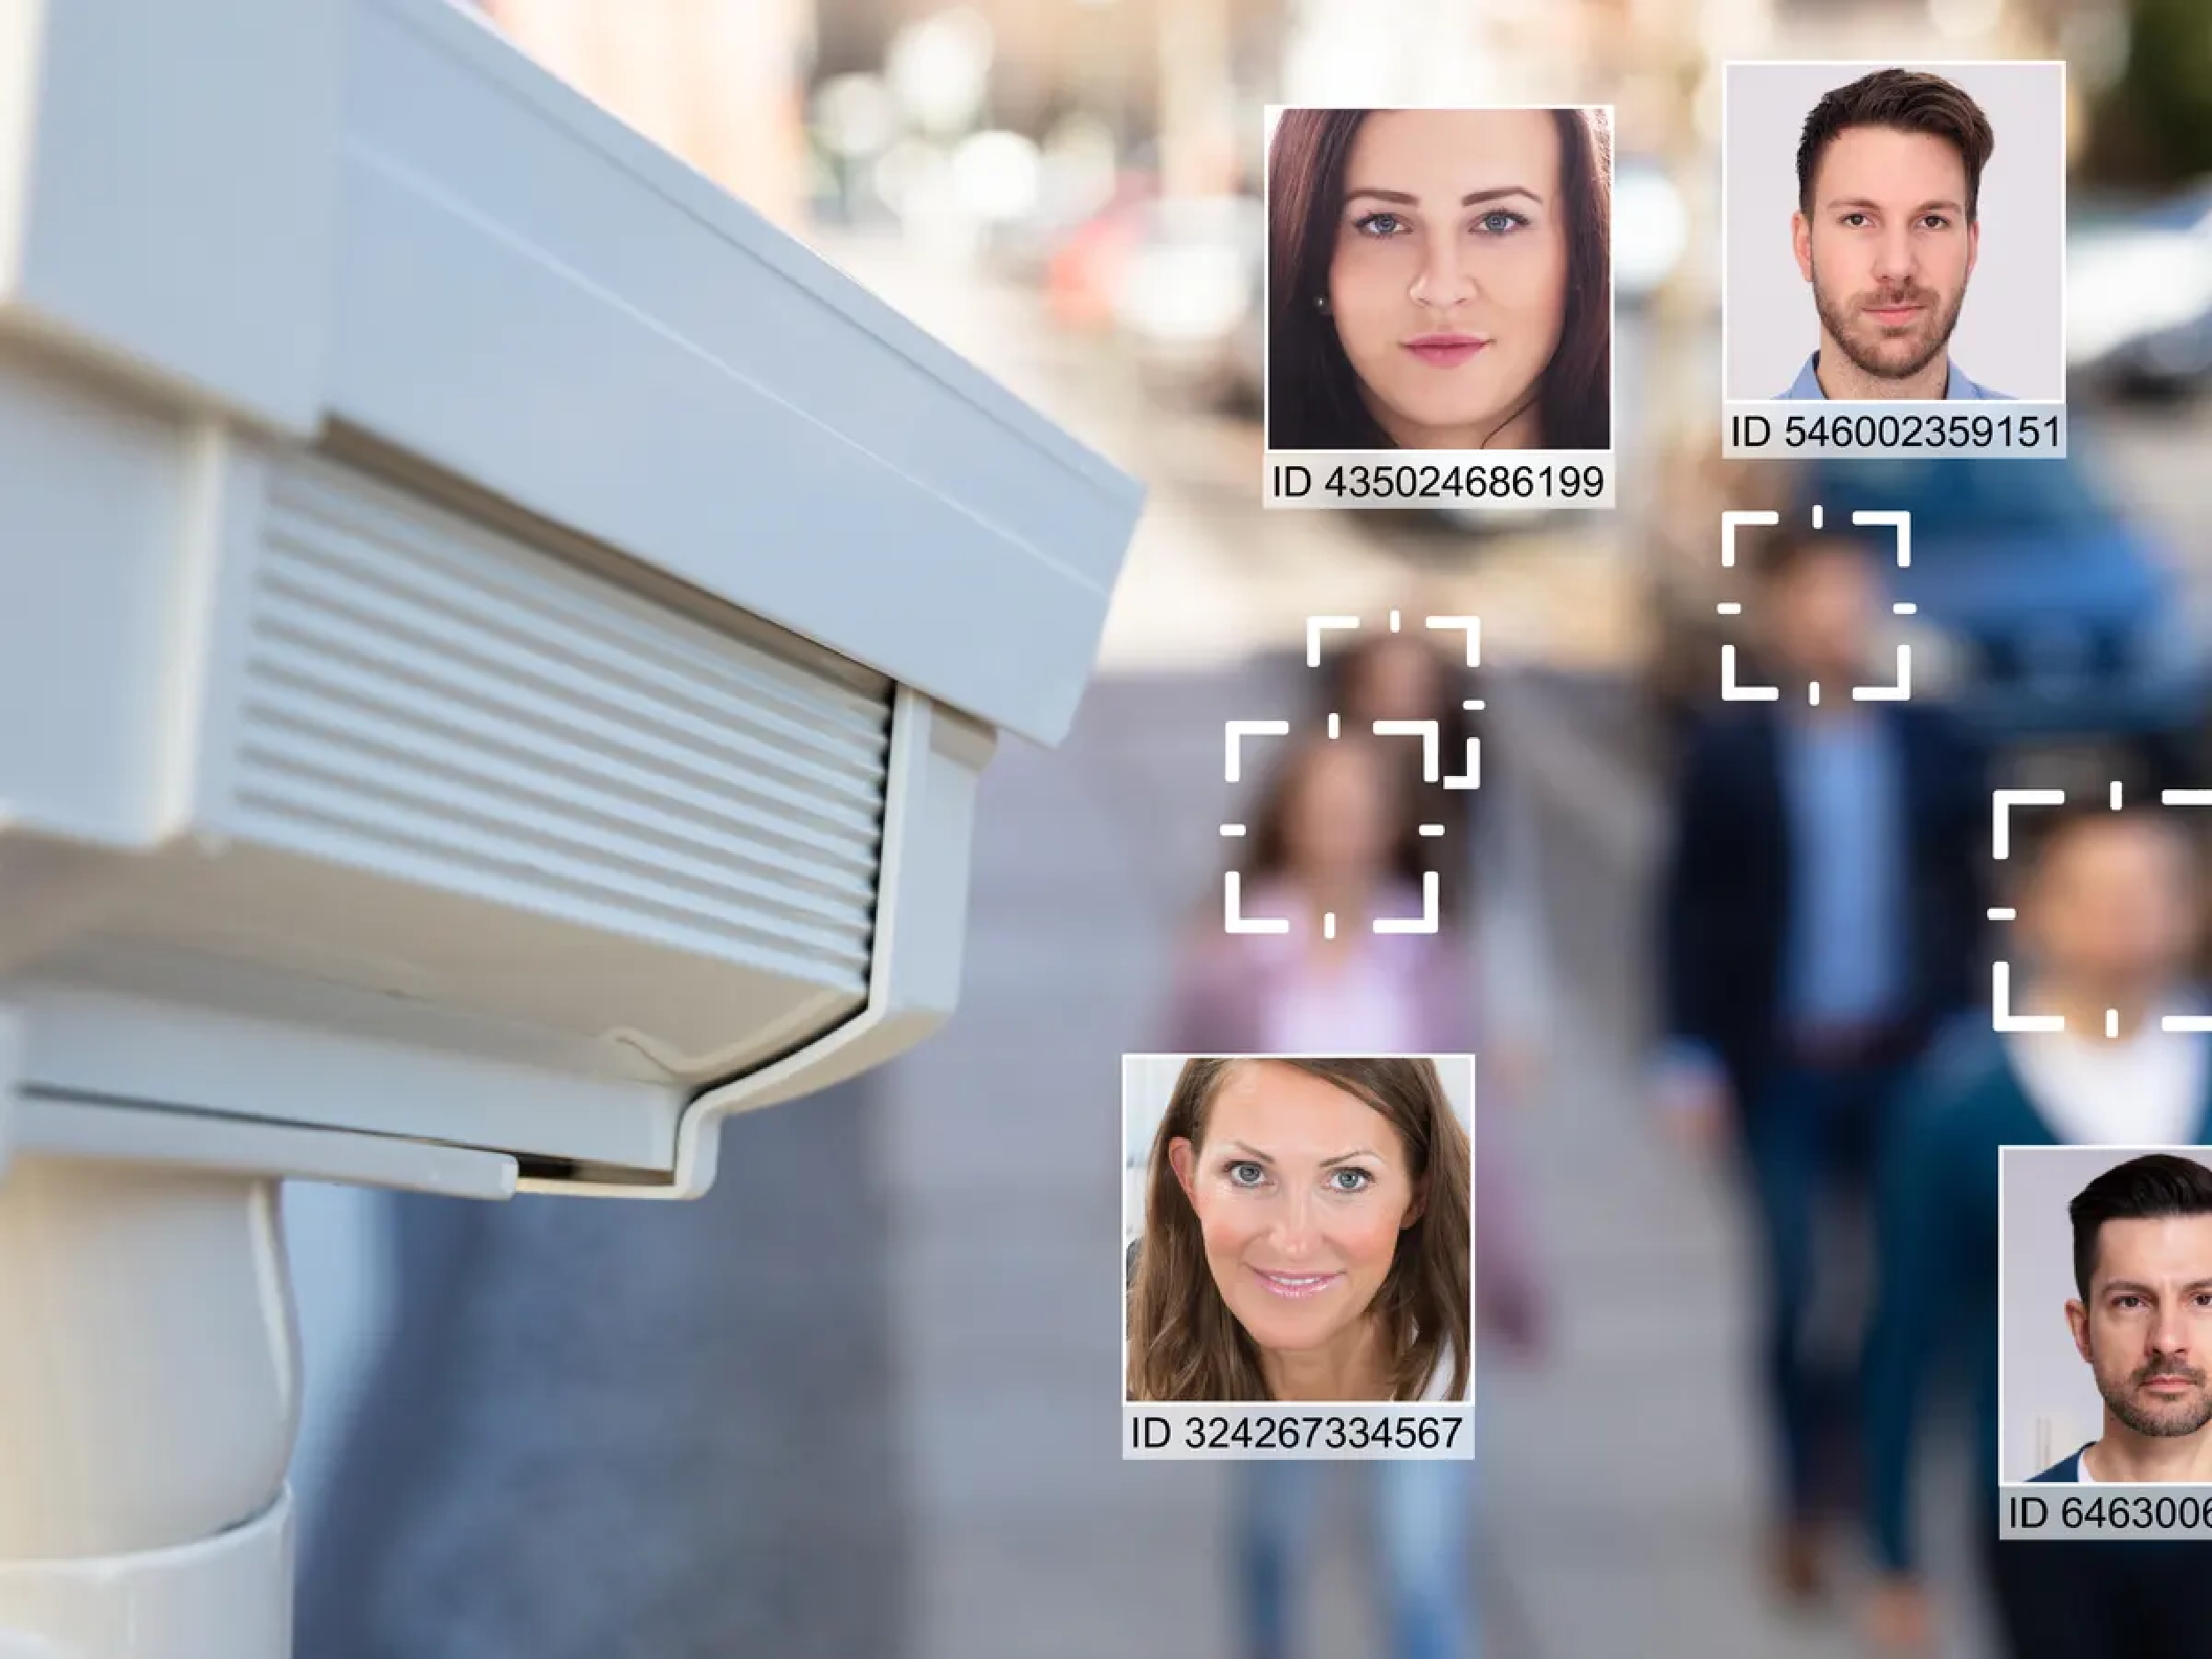
\includegraphics[height=3cm]{../illustrations/camera}
    \hspace{1cm}
  \end{figure}
  \pdfcomment[icon=Note]{Différents secteurs de l'industrie (lourde, des lignes de recyclage des déchets, au GAFAM sur internet, en passant le médical et le spatial)}
  \pdfcomment[icon=Note]{   }
  \pdfcomment[icon=Note]{Différents appareils (des ordinateurs/téléphones aux machines lourdes, en passant par James Webb et les IRM)}
  \pdfcomment[icon=Note]{   }
  \pdfcomment[icon=Note]{Différentes applications (retoucher ses photos, reconnaître des visages, appliquer des filtres snapshats, trouver des tumeurs, trouver des étoiles)}
  \pdfcomment[icon=Note]{   }
  \pdfcomment[icon=Note]{Le traitement d'image coûte des ressources !}
  \pnote{
    Différents secteurs de l'industrie (lourde, des lignes de recyclage des déchets, au GAFAM sur internet, en passant le médical et le spatial)

    Différents appareils (des ordinateurs/téléphones aux machines lourdes, en passant par James Webb et les IRM)

    Différentes applications (retoucher ses photos, reconnaître des visages, appliquer des filtres snapshats, trouver des tumeurs, trouver des étoiles)

    Le traitement d'image coûte des ressources !
  }
\end{frame}

\begin{frame}[fragile]{Image processing nowadays}
  \begin{alertblock}{Different data types and algorithms}
    \begin{itemize}
      \item image-ND, hexagonal grid, cubical complexes value, etc.
      \item pixel-wise algorithms, local algorithms (convolution), global algorithms (propagation)
    \end{itemize}
  \end{alertblock}
  \begin{figure}[bl]
    \centering
    \hfill
    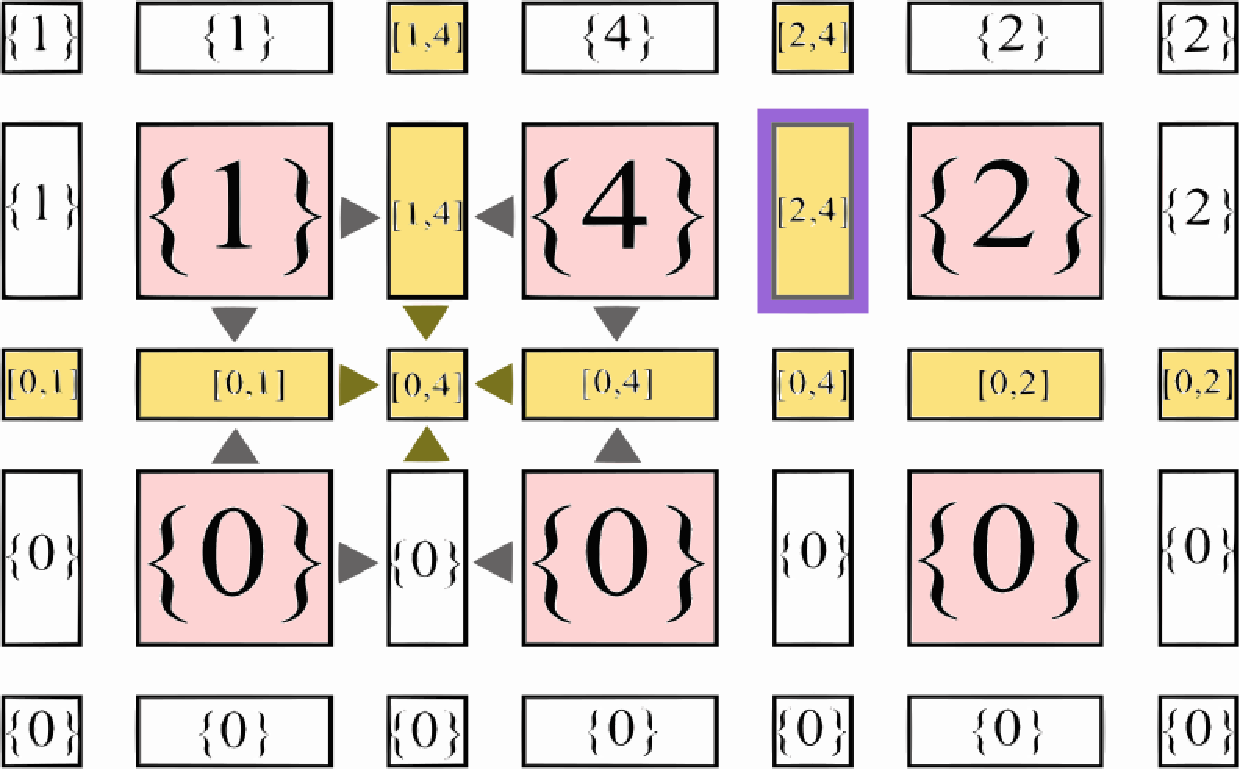
\includegraphics[height=2.3cm]{../illustrations/cubical_complex}
    \hfill
    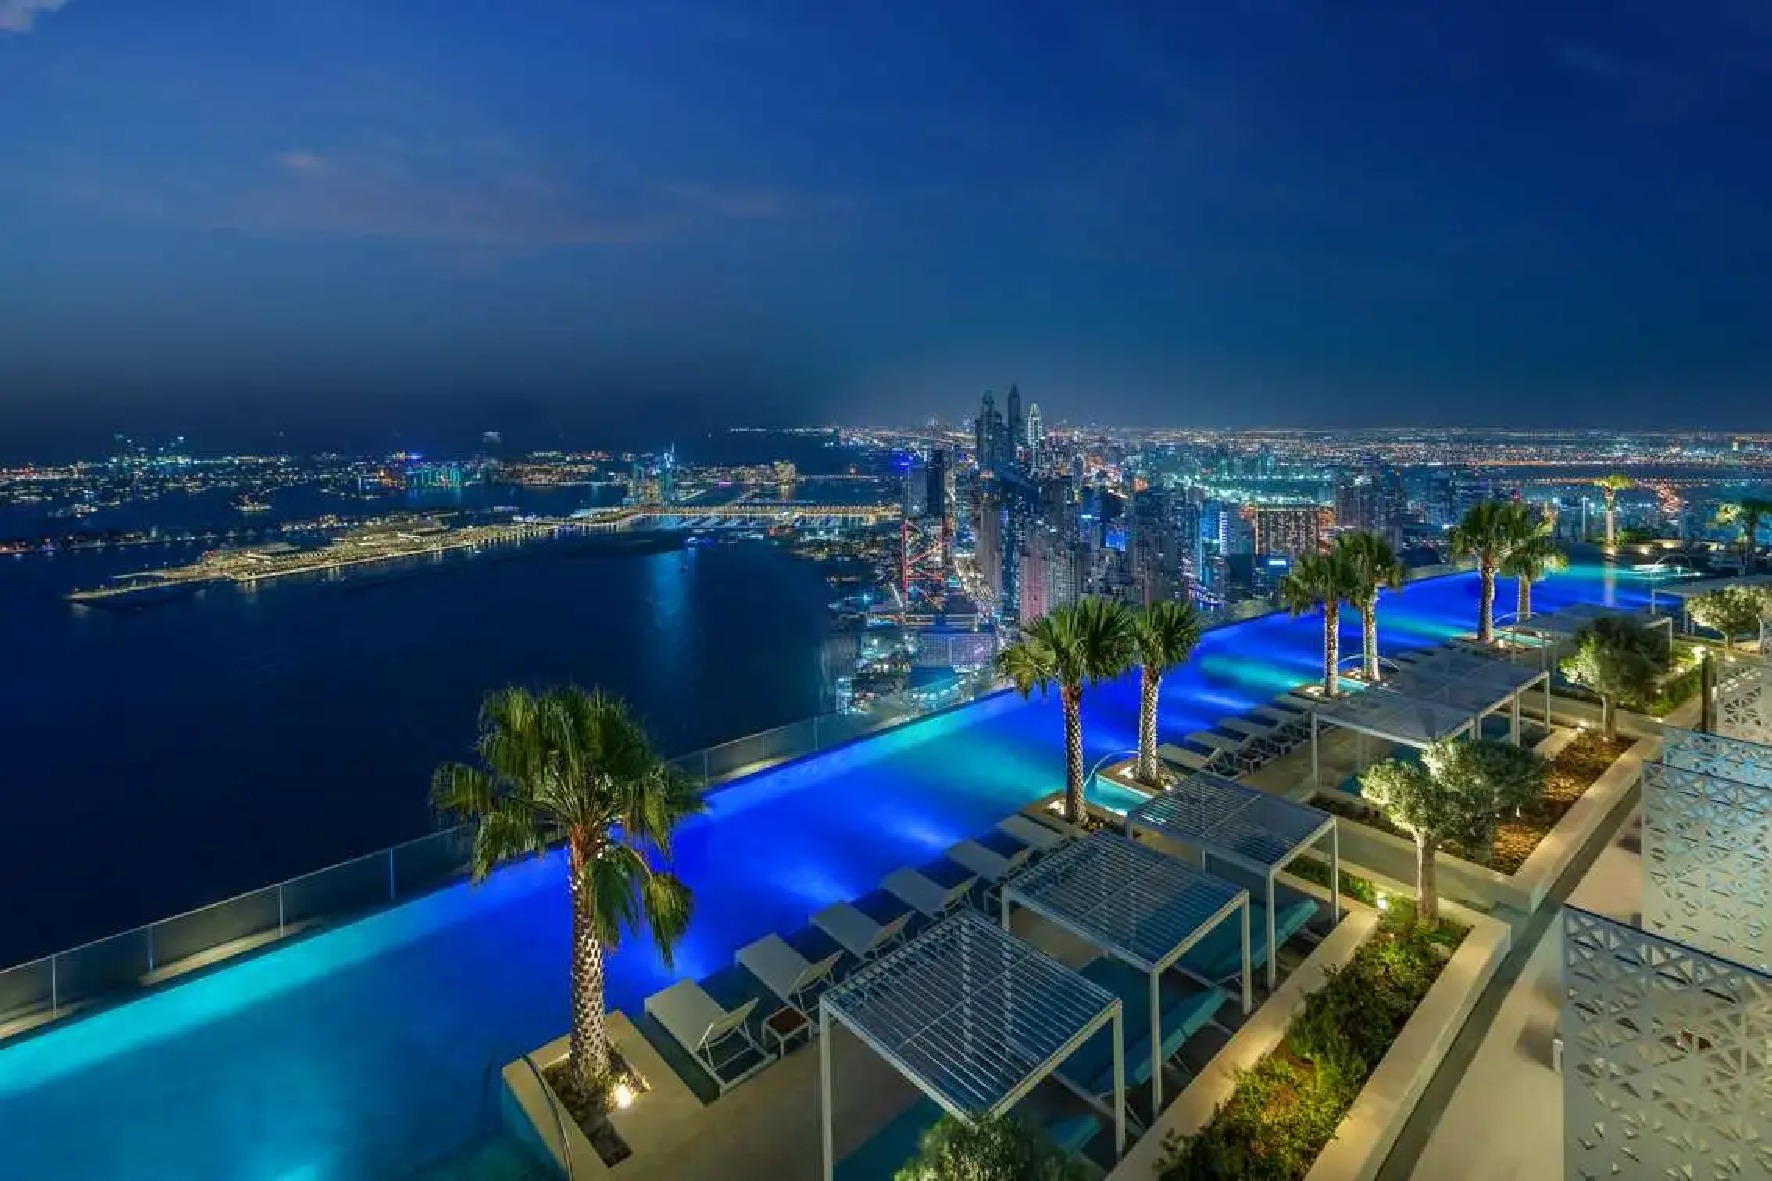
\includegraphics[height=2.3cm]{../illustrations/2d_rgb8_holiday_image}
    \hfill
    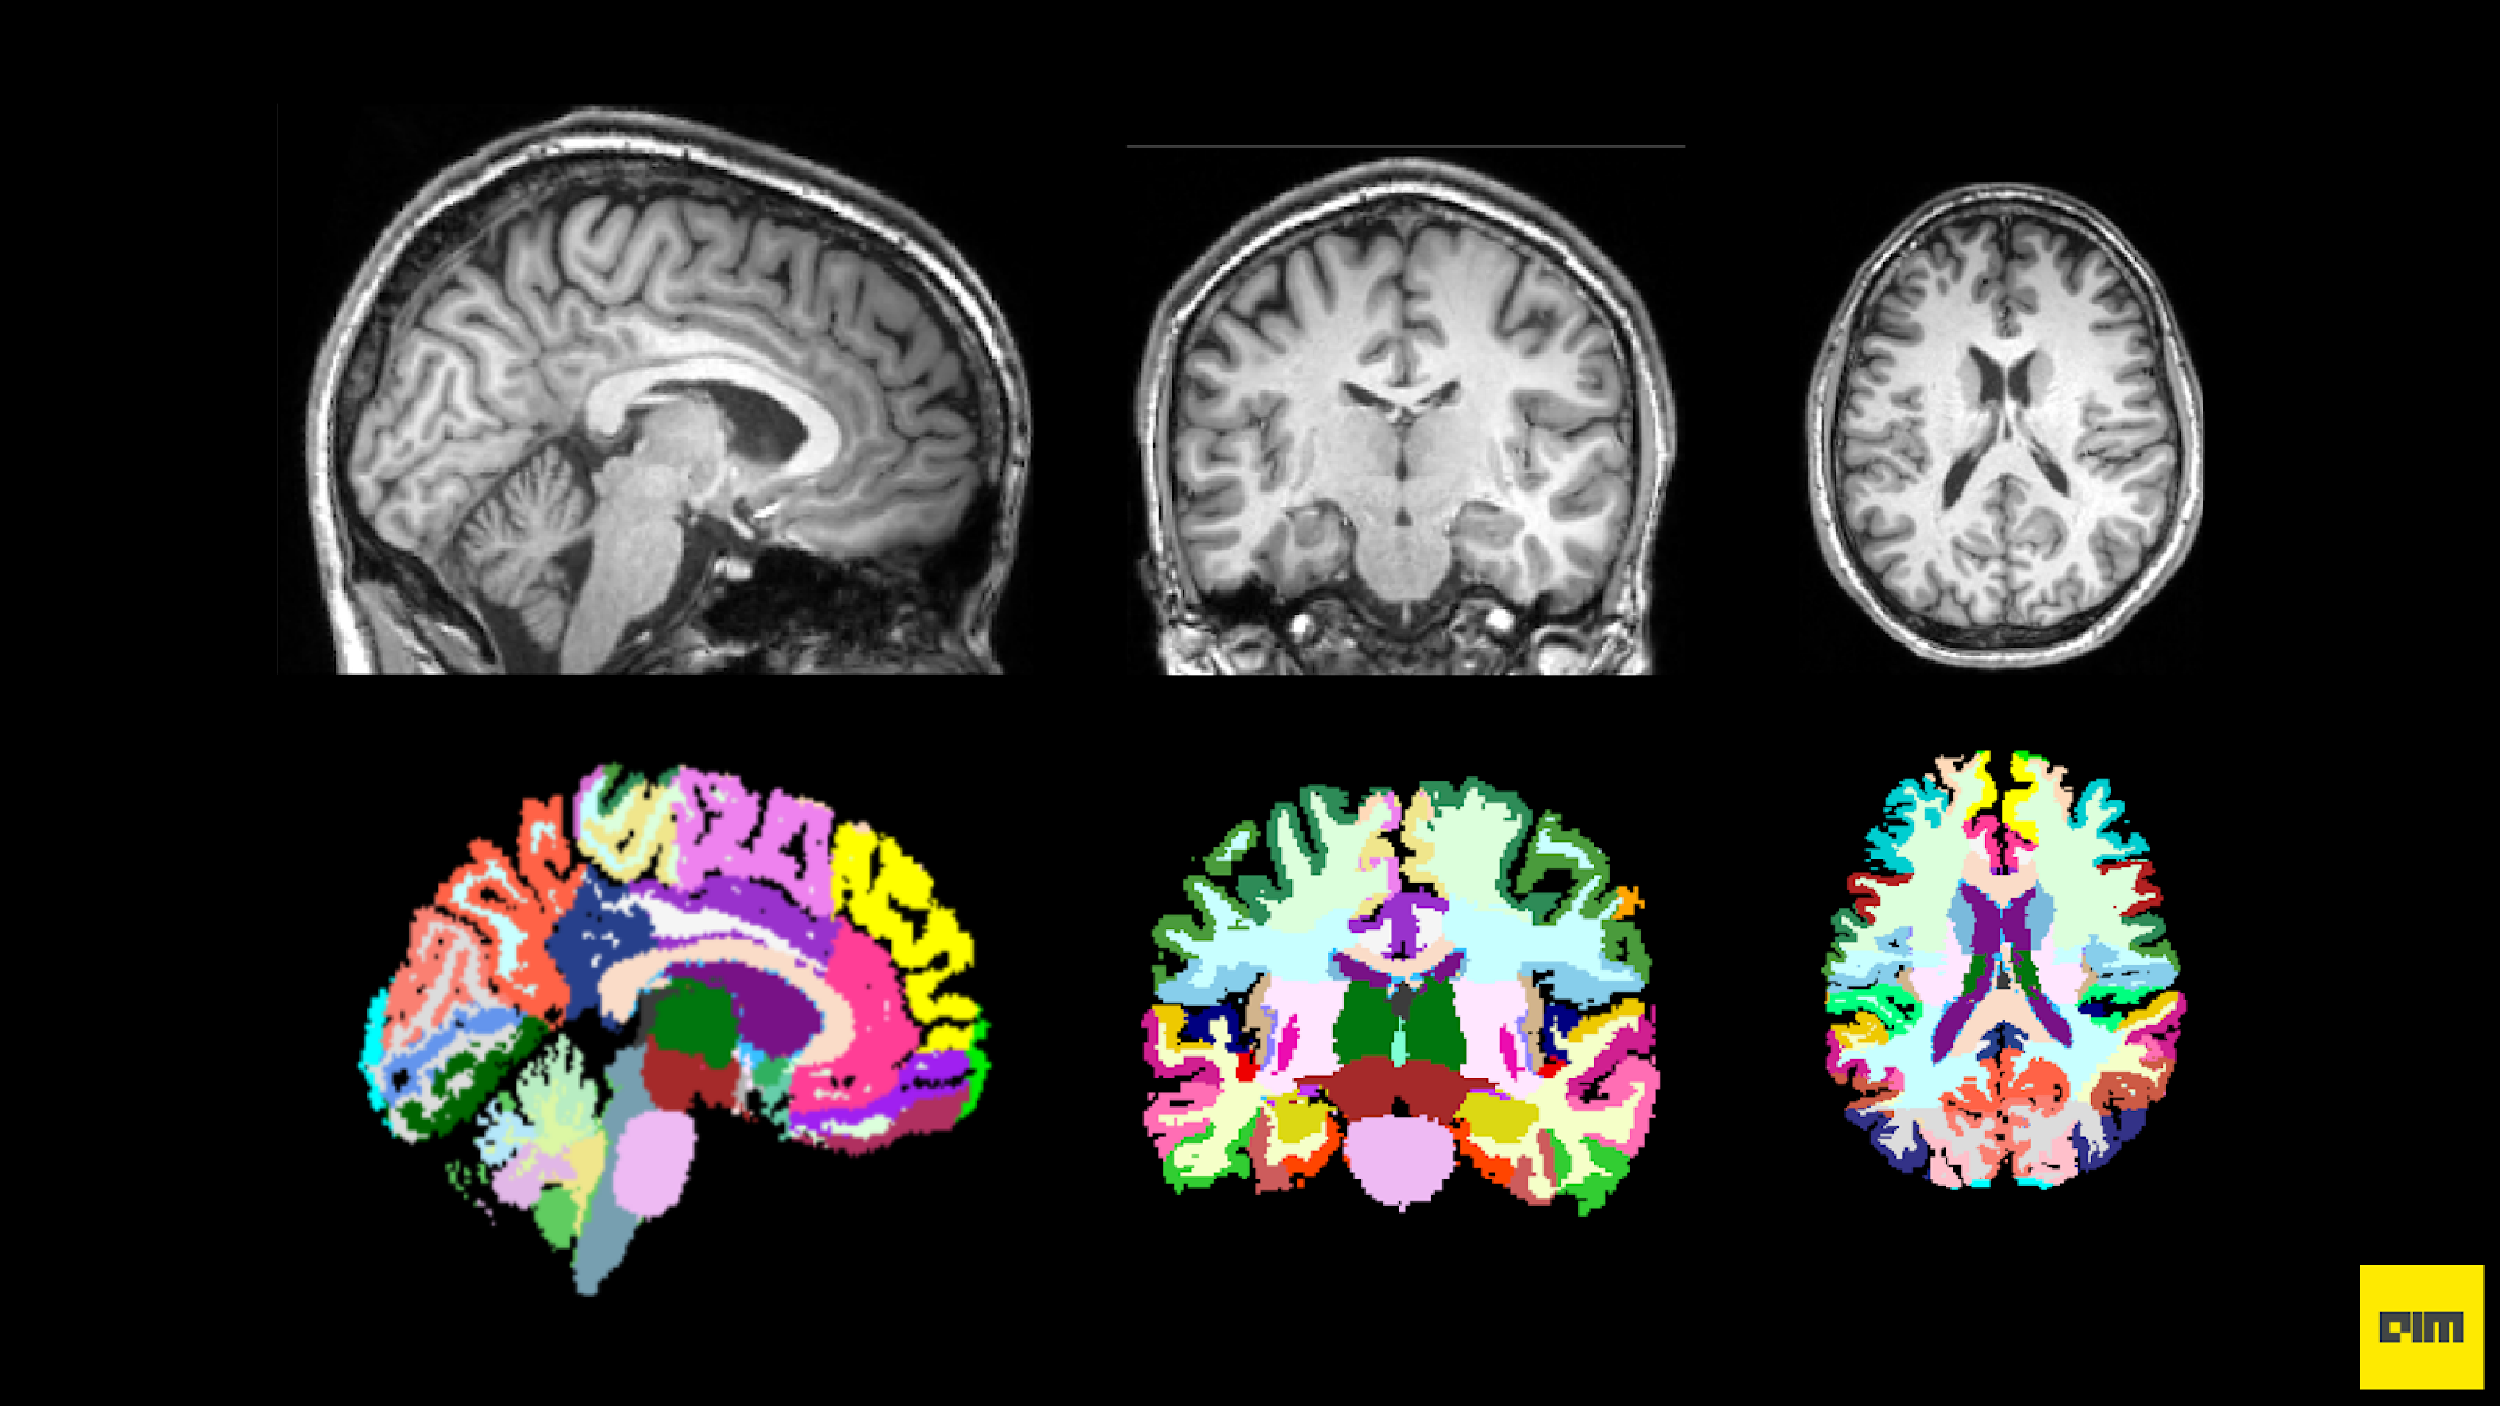
\includegraphics[height=2.3cm]{../illustrations/3d_medical_image}
    \hfill
    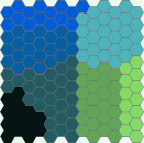
\includegraphics[height=2.3cm]{../illustrations/hexagonal_grid2}
    \hspace{1cm}
  \end{figure}
  \pdfcomment[icon=Note]{Différents domaines/applications/appareils -> différents besoin -> différents types de données / façon de modéliser ses données}
  \pdfcomment[icon=Note]{   }
  \pdfcomment[icon=Note]{Image 2D classique pour la reconnaissance}
  \pdfcomment[icon=Note]{Images 3D pour le médical}
  \pdfcomment[icon=Note]{Images graph, image complex cubique etc.}
  \pnote{
    Différents domaines/applications/appareils -> différents besoin -> différents types de données / façon de modéliser ses données

    Image 2D classique pour la reconnaissance
    Images 3D pour le médical
    Images graph, image complex cubique etc.
  }
\end{frame}

\begin{frame}[fragile]{Image processing nowadays}
  \begin{alertblock}{Different user profiles and their use cases}
    \begin{itemize}
      \item The end user \GRAYOUT{(non-programmer, wants UI interface).}
      \item The practitioner \GRAYOUT{(end user of an image processing library).}
      \item The contributor \GRAYOUT{(advanced user of a library familiar with its internals).}
      \item The maintainer \GRAYOUT{(founder/creator of the library or took it over to make it grow).}
    \end{itemize}
  \end{alertblock}

  Our work is aimed toward the \emph{practitioner}, the \emph{contributor} and the \emph{maintainer}.
  \pdfcomment[icon=Note]{Différents types d'utilisateurs}
  \pdfcomment[icon=Note]{   }
  \pdfcomment[icon=Note]{L'utilisateur final veut une interface graphique pour retoucher ses photos ou utiliser une application riche (snapchat, instagram) qui embarque les fonctionnalités dont il a besoin}
  \pdfcomment[icon=Note]{   }
  \pdfcomment[icon=Note]{Le praticien veut des bibliothèques accessibles et documenter et travailler dans des environnements où on peut itérer rapidement pour développer son application complexe}
  \pdfcomment[icon=Note]{   }
  \pdfcomment[icon=Note]{Le contributeur veut pouvoir mettre les mains dans les détails interne d'une bibliothèque pour implémenter ses algorithmes et répondre aux besoin, par exemple, d'un praticien}
  \pdfcomment[icon=Note]{   }
  \pdfcomment[icon=Note]{Le mainteneur se charge de faire vivre une bibliothèque de TI dans le temps, donc d'implémenter les nouveaux algorithmes de l'état de l'art au fur et à mesure du temps}
  \pnote{
    Différents types d'utilisateurs

    L'utilisateur final veut une interface graphique pour retoucher ses photos ou utiliser une application riche (snapchat, instagram) qui embarque les fonctionnalités dont il a besoin

    Le praticien veut des bibliothèques accessibles et documenter et travailler dans des environnements où on peut itérer rapidement pour développer son application complexe

    Le contributeur veut pouvoir mettre les mains dans les détails interne d'une bibliothèque pour implémenter ses algorithmes et répondre aux besoin, par exemple, d'un praticien

    Le mainteneur se charge de faire vivre une bibliothèque de TI dans le temps, donc d'implémenter les nouveaux algorithmes de l'état de l'art au fur et à mesure du temps
  }
\end{frame}

\begin{frame}[fragile]{Image processing nowadays}
  \begin{alertblock}{Different tools}
    \begin{itemize}
      \item Graphic editors \GRAYOUT{(GIMP, Photoshop).}
      \item Command line utilities \GRAYOUT{(ImageMagick, GraphicsMagick or MegaWave).}
      \item Visual programming environment \GRAYOUT{(Mathcad).}
      \item Integrated environment \GRAYOUT{(Matlab, Scilab, Octave, Mathematica and Jupyter).}
      \item Package for Python \GRAYOUT{(SciPy, NumPy, Scikit-image, Pillow or OpenCV bindings, via PyPi or Conda).}
      \item \hl{Programming libraries} \GRAYOUT{(IPP, ITK, Boost.GIL, Vigra, Higra, GrAL, DGTal, OpenCV, CImg, Video++,
              Generic Graphic Library, Milena and Pylena).}
      \item Domain Specific Languages (DSL) \GRAYOUT{(Eigen, Blaze, Blitz++ or Armadillo via C++ Expression template, or
              Halide and SYCL with their own toolchain).}
    \end{itemize}
  \end{alertblock}
  \pdfcomment[icon=Note]{Différents outils pour différents utilisateurs}
  \pdfcomment[icon=Note]{   }
  \pdfcomment[icon=Note]{Outils de programmation intégrés et visuels, pour le patricien}
  \pdfcomment[icon=Note]{Packages dynamiques pour le patricien}
  \pdfcomment[icon=Note]{   }
  \pdfcomment[icon=Note]{Bibliothèque de TI pour le contributeur (pour les faire évoluer, ou les packager pour les langages dynamiques pour la patricien)}
  \pdfcomment[icon=Note]{   }
  \pdfcomment[icon=Note]{DSL permet d'exprimer son problème, dans un langage de programmation, son problème pour qu'il soit ensuite résolu par le compilateur qui le transforme en code compréhensible pour la machine.
    Utilisé par écrire des équations d'algèbre via frameworks type Eigen ou Armadillo).}
  \pdfcomment[icon=Note]{Utilisé pour abstraire la couche architecture et faire de la programmation hétérogène dans Halide et et les langages implémentant le standard SYCL.}
  \pnote{
    Différents outils pour différents utilisateurs

    Outils graphique et en ligne de commande pour l'utilisateur final

    Outils de programmation intégrés et visuels, pour le patricien
    Packages dynamiques pour le patricien

    Bibliothèque de TI pour le contributeur (pour les faire évoluer, ou les packager pour les langages dynamiques pour la patricien)

    DSL permet d'exprimer son problème, dans un langage de programmation, son problème pour qu'il soit ensuite résolu par le compilateur qui le transforme en code compréhensible pour la machine.
    Utilisé par écrire des équations d'algèbre via frameworks type Eigen ou Armadillo). Utilisé pour abstraire la couche architecture et faire de la programmation hétérogène dans Halide et et les langages implémentant le standard SYCL.
  }
\end{frame}

\begin{frame}[fragile]{Need of Genericity for image processing}
  \begin{figure}[htbp]
    \raggedright\small
    \begin{tabular}{cccc}
                                                                              & image 2D
                                                                              & graph    & mesh \\[5pt]
      input:                                                                  &
      \fbox{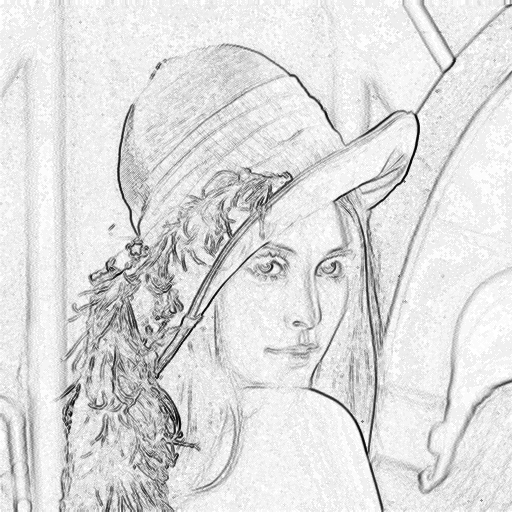
\includegraphics[width=.14\linewidth]{../figures/geninput-000b}}  &
      \fbox{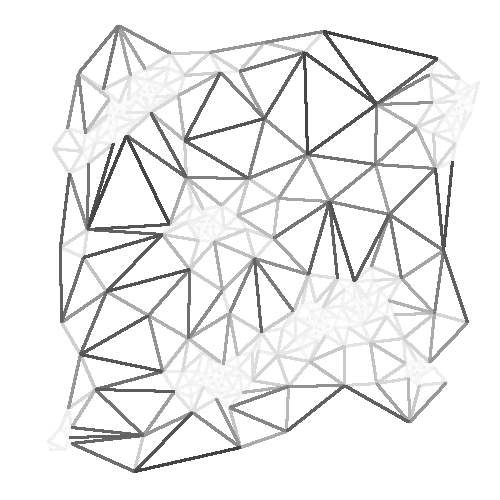
\includegraphics[width=.14\linewidth]{../figures/geninput-001b}}  &
      \fbox{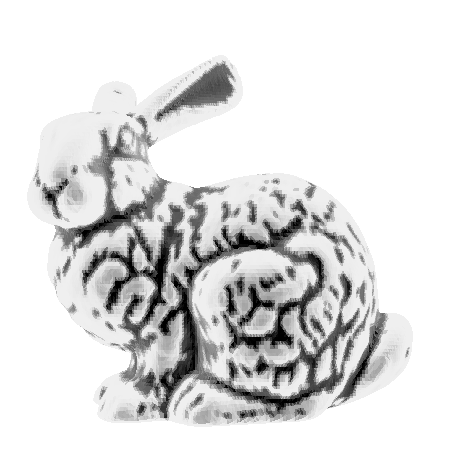
\includegraphics[width=.14\linewidth]{../figures/geninput-002b}}
      \\[5pt]
      %
      output:                                                                 &
      \fbox{
\includegraphics[width=.14\linewidth]{../figures/genoutput-000}}  &
      \fbox{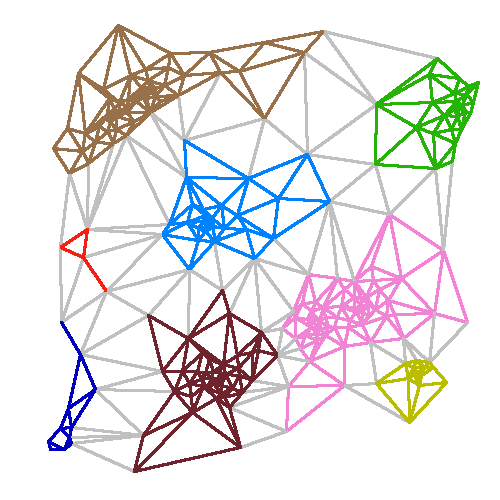
\includegraphics[width=.14\linewidth]{../figures/genoutput-001b}} &
      \fbox{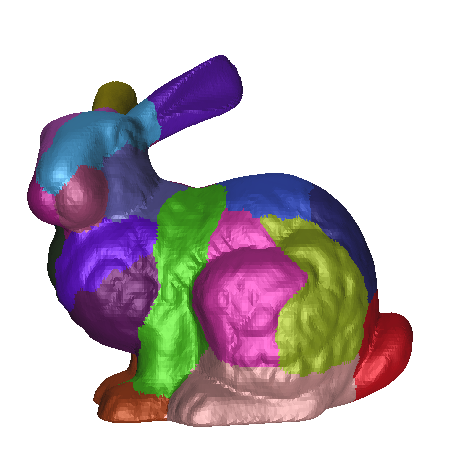
\includegraphics[width=.14\linewidth]{../figures/genoutput-002b}}
      \\
    \end{tabular}
    \label{fig:type.vs.algo}
    \caption{Watershed algorithm applied to three different image types.~\footnote{Levillain et al., Practical
        genericity: Writing image processing algorithms both reusable and efficient. CIARP, 2014}}
    %\vspace{-0.5cm}
    %\text{\textbf{Algorithms are intrinsically generics.}}
  \end{figure}
  \begin{textblock*}{4cm}(11cm,4cm)
    \textbf{Algorithms are intrinsically generic.}
  \end{textblock*}
  \pdfcomment[icon=Note]{On se retrouve avec une multitudes de domaines d'applications, de périphériques, d'utilisateurs, de type de bibliothèque, et bien entendu, d'algorithmes.}
  \pdfcomment[icon=Note]{   }
  \pdfcomment[icon=Note]{Les algorithmes ne sont pas spécifiques à un seul type d'image ou de valeurs, mais sont intrinsèquement générique.}
  \pdfcomment[icon=Note]{   }
  \pdfcomment[icon=Note]{Par ex: watershed = ligne de partage des eaux = algorithme de segmentation qui va considérer tous les niveaux de gris d'une image comme du relief topographique pour extraire les régions.}
  \pdfcomment[icon=Note]{   }
  \pdfcomment[icon=Note]{L'expression de cet algorithme est censée marcher sur imageND, mesh, graphs etc.}
  \pdfcomment[icon=Note]{Seul l'implémentation contraint la structure de donnée et ce n'est pas justifié.}
  \pdfcomment[icon=Note]{On a donc un besoin d'implémenter notre algorithem de manière générique pour qu'il fonctionne sur tous les types d'image.}
  \pnote{
    On se retrouve avec une multitudes de domaines d'applications, de périphériques, d'utilisateurs, de type de bibliothèque, et bien entendu, d'algorithmes.

    Les algorithmes ne sont pas spécifiques à un seul type d'image ou de valeurs, mais sont intrinsèquement générique.

    Par ex: watershed = ligne de partage des eaux = algorithme de segmentation qui va considérer tous les niveaux de gris d'une image comme du relief topographique pour extraire les régions.

    L'expression de cet algorithme est censée marcher sur imageND, mesh, graphs etc.
    Seul l'implémentation contraint la structure de donnée et ce n'est pas justifié.
    On a donc un besoin d'implémenter notre algorithem de manière générique pour qu'il fonctionne sur tous les types d'image.
  }
\end{frame}

% levillain.2014.ciarp
% Levillain, R., Géraud, T., Najman, L., & Carlinet, E. (2014). Practical genericity: Writing image processing
% algorithms both reusable and efficient. In E. Bayro & E. Hancock (Eds.), Progress in pattern recognition, image
% analysis, computer vision, and applications - proceedings of the 19th iberoamerican congress on pattern recognition
% (ciarp) (pp. 70–79, Vol. 8827). Springer-Verlag. (Cit. on p. 8).

\begin{frame}[fragile]{Need of Genericity for image processing}
  Algorithm must support combination whose cardinality increases with:

  \begin{columns}[T,onlytextwidth]
    \column{0.52\textwidth}
    \begin{itemize}
      \item supported underlying image value type (grayscale, rgb, floating-point, \ldots)
      \item supported data structure (ND-buffers, graphs, meshes, \ldots)
      \item additional data type (structuring element, masks, \ldots)
    \end{itemize}

    \column{0.47\textwidth}
    \begin{figure}[htbp]
      \centering
      \includegraphics[width=0.7\textwidth]{../figures/possibility_space}
      \caption{Space of possibilities.}
      \label{fig:int.possibility_space}
    \end{figure}
  \end{columns}

  \begin{alertblock}{What is a generic algorithm?}
    An algorithm is generic when it is written once to perform over a wide array of data structures.
  \end{alertblock}
  \pdfcomment[icon=Note]{En effet, un algorithme non-générique a son implémentation qui grossit en complexité en fonction de tous les types de données d'entré qu'il doit gérer.}
  \pdfcomment[icon=Note]{Données qui peuvent être relatives à la dimension, la représentation (grille rectangle, hexa, graphe), le type sous-jascentes des valeurs des pixels (rgb, niveau de gris, floatant, bool) et les structures auxiliaries (élément structurant, valeurs de seuil, labels, etc.)}
  \pdfcomment[icon=Note]{   }
  \pdfcomment[icon=Note]{espace des possibilités surface -> volume (avec structures auxiliaires).}
  \pdfcomment[icon=Note]{   }
  \pdfcomment[icon=Note]{--> On dit qu'un algorithme est générique lorsqu'il a une seule implémentation qui va fonctionner pour un large éventails de structures de données.}
  \pnote{
    En effet, un algorithme non-générique a son implémentation qui grossit en complexité en fonction de tous les types de données d'entré qu'il doit gérer.
    Données qui peuvent être relatives à la dimension, la représentation (grille rectangle, hexa, graphe), le type sous-jascentes des valeurs des pixels (rgb, niveau de gris, floatant, bool) et les structures auxiliaries (élément structurant, valeurs de seuil, labels, etc.)

    espace des possibilités surface -> volume (avec structures auxiliaires)

    ---> On dit qu'un algorithme est générique lorsqu'il a une seule implémentation qui va fonctionner pour un large éventails de structures de données.
  }
\end{frame}

%
%
%

% \AtBeginSection[]
% {
%   \begin{frame}{Outline}
%     \setbeamertemplate{section in toc}[sections numbered]
%     \vspace{0.2cm}
%     \small%\singlespacing
%     \tableofcontents[currentsection]
%   \end{frame}
% }

\section[Context and history of generic programming]{Context and history of generic programming}

\begin{frame}{Outline}
  \setbeamertemplate{section in toc}[sections numbered]
  \vspace{0.2cm}
  \small%\singlespacing
  \tableofcontents[currentsection]
  \pdfcomment[icon=Note]{Maintenant que nous avons vu le besoin de généricité des algorithmes de traitement d'image, passons à comment nous pouvons rendre générique un algorithme de traitement d'image.}
  \pdfcomment[icon=Note]{   }
  \pdfcomment[icon=Note]{--> 8min <--}
  \pnote{
    Maintenant que nous avons vu le besoin de généricité des algorithmes de traitement d'image, passons à comment nous pouvons rendre générique un algorithme de traitement d'image.

    --> 8min <--
  }
\end{frame}

\subsection[Unconstrained Genericity]{Unconstrained Genericity}

\begin{frame}[fragile]{Non-generic algorithm: gamma correction}
  Introducing the process of (generic) \textbf{Generalization}~\footnote{Roynard et al., An image processing library in
    modern C++: Getting simplicity and efficiency with generic programming. RRPR, 2019}. \\
  Non-generic gamma-correction algorithm:
  \vspace{-0.3cm}
  \begin{minted}[linenos]{C++}
    void gamma_correction(Image& ima, double gamma)
    {
      const auto gamma_corr = 1.f / gamma;
      for (int x = 0; x < ima.width(); ++x)
        for (int y = 0; y < ima.height(); ++y)
        {
          ima(x, y).r = 256.f * std::pow(ima(x, y).r / 256.f, gamma_corr);
          ima(x, y).g = 256.f * std::pow(ima(x, y).g / 256.f, gamma_corr);
          ima(x, y).b = 256.f * std::pow(ima(x, y).b / 256.f, gamma_corr);
        }
    }
  \end{minted}
  \begin{textblock*}{4cm}(11cm,1.5cm)
    This algorithm is \textbf{over-constrained}. \\
    How can we make it \textbf{Generic}?
  \end{textblock*}
  \pdfcomment[icon=Note]{Prenons par exemple l'algorithme de correction gamma}
  \pdfcomment[icon=Note]{   }
  \pdfcomment[icon=Note]{Cet algorithme fait une double boucle (2D)}
  \pdfcomment[icon=Note]{Il corrige notre triplet RGB en nombre flottant en supposant que la valeur max ici est 256.}
  \pdfcomment[icon=Note]{   }
  \pdfcomment[icon=Note]{Cette algorithme est sur-contraint et ce n'est pas justifié.}
  \pdfcomment[icon=Note]{   }
  \pdfcomment[icon=Note]{Essayons d'abord plusieurs approches pour rendre cette algorithme générique = Comment on le généralise}
  \pnote{
    Prenons par exemple l'algorithme de correction gamma

    Cet algorithme fait une double boucle (2D)
    Il corrige notre triplet RGB en nombre flottant en supposant que la valeur max ici est 256.

    Cette algorithme est sur-contraint et ce n'est pas justifié.

    Essayons d'abord plusieurs approches pour rendre cette algorithme générique = Comment on le généralise
  }
\end{frame}

% roynard.2019.rrpr
% Roynard, M., Carlinet, E., & Géraud, T. (2019). An image processing library in modern C++: Getting simplicity and
% efficiency with generic programming. In B. Kerautret, M. Colom, D. Lopresti, P. Monasse, & H. Talbot (Eds.),
% Reproducible research in pattern recognition (pp. 121–137). Springer International Publishing. (Cit. on pp. 11, 54).

\begin{frame}[fragile]{1rst approach: Code duplication}
  \begin{itemize}
    \item Writing and optimizing an algorithm for a particular data type in mind.
    \item Often results in multiple switch/cases to enumerate all the supported combination of supported data types.
  \end{itemize}
  \begin{minted}{C++}
    void gamma_correction(any_image img, double gamma)
    {
      switch((img.structure_kind, img.value_kind)) 
      {
      case (BUFFER2D, UINT8):
        gamma_correction_img2d_uint8( (image2d<uint8>) img, gamma );
      // ...
      case (LUT, RGB8):
        gamma_correction_lut_rgb8( (image_lut<rgb8>) img, gamma );
      // ...
      }
    }
  \end{minted}
  \pdfcomment[icon=Note]{Première approche, naive.}
  \pdfcomment[icon=Note]{   }
  \pdfcomment[icon=Note]{On écrit un algorithme car combinaison de structure de données puis on dispatch depuis l'algorithme "générique" dans un grand switch case.}
  \pdfcomment[icon=Note]{   }
  \pdfcomment[icon=Note]{Devient très rapidement un enfer à maintenantir. Pas viable sur le long terme.}
  \pnote{
    Première approche, naive.

    On écrit un algorithme car combinaison de structure de données puis on dispatch depuis l'algorithme "générique" dans un grand switch case.
    Devient très rapidement un enfer à maintenantir. Pas viable sur le long terme.
  }
\end{frame}

\begin{frame}[fragile]{2nd approach: Generalization}
  \begin{itemize}
    \item Necessity to have a common denominator to all the supported types:\\
          \hl{the super-type}.
    \item All supported data types must be convertible to and from this super-type.
    \item Good for maintenance but conversions impact performance.
  \end{itemize}
  \begin{minted}{C++}
    struct image4D { // generalized super-type with generalized underlying value-type
      using value_type = std::array<double, 4>; // every value is converted to this one
    }; // specific types w/ conversion routines
    struct image2D { image4D to(); void from(image4D); };
    struct image3D { image4D to(); void from(image4D); };
    void gamma_correction(image4D ima, double gamma) {
      for(auto t : ima.time())
        for(auto z : ima.depth())
          for(auto y : ima.width())
            for(auto x : ima.height())
              auto& v = ima(x, y, z, t); // image4D::value_type
              // correct v with gamma
    }
  \end{minted}
  \pdfcomment[icon=Note]{Deuxième approche: la généralisation (au sens super-type).}
  \pdfcomment[icon=Note]{   }
  \pdfcomment[icon=Note]{On fait en sorte que tous nos types supportées soit convertibles vers et depuis ce super-type.}
  \pdfcomment[icon=Note]{On écrit une fois l'algorithme pour le super-type.}
  \pdfcomment[icon=Note]{   }
  \pdfcomment[icon=Note]{Très intéressant côté maintenance.}
  \pdfcomment[icon=Note]{Pertes d'opportunités d'optimisations (ex ici 4 boucles alors que image 1d = 1 boucle).}
  \pnote{
    Deuxième approche: la généralisation (au sens super-type).

    On fait en sorte que tous nos types supportées soit convertibles vers et depuis ce super-type.
    On écrit une fois l'algorithme pour le super-type

    Très intéressant côté maintenance
    Pertes d'opportunités d'optimisations (ex ici 4 boucles alors que image 1d = 1 boucle)
  }
\end{frame}

\begin{frame}[fragile]{Toward Genericity: Step 1}
  Lifting RGB constraint:
  \begin{minted}[linenos,highlightlines={3,6,10},highlightcolor=yellow!60!white]{C++}
    void gamma_correction(Image& ima, double gamma)
    {
      using value_t = typename Image::value_type;

      const auto gamma_corr = 1.f / gamma;
      const auto max_val = std::numeric_limits<value_t>::max();
    
      for(int x = 0; x < ima.width(); ++x)
        for(int y = 0; y < ima.height(); ++y)
          ima(x, y) = max_val * std::pow(ima(x, y) / max_val, gamma_corr);
    }
  \end{minted}
  \begin{textblock*}{4cm}(11.5cm,1.5cm)
    \textbf{There is no valid reason to constrain this algorithm to RGB images.}
  \end{textblock*}
  \pdfcomment[icon=Note]{Essayons maintenant une autre façon d'écrire notre algorithme pour qu'il ne soit plus sur-contraint et devienne générique.}
  \pdfcomment[icon=Note]{   }
  \pdfcomment[icon=Note]{Aucune raison pour qu'il ne fonctionne qu'avec les images rgb flotantes.}
  \pdfcomment[icon=Note]{   }
  \pdfcomment[icon=Note]{Nous le réécrivons de façon à abstraire les opérations sur la valeur des pixels de l'image.}
  \pnote{
    Essayons maintenant une autre façon d'écrire notre algorithme pour qu'il ne soit plus sur-contraint et devienne générique.

    Aucune raison pour qu'il ne fonctionne qu'avec les images rgb flotantes.

    Nous le réécrivons de façon à abstraire les opérations sur la valeur des pixels de l'image
  }
\end{frame}

\begin{frame}[fragile]{Toward Genericity: Step 2}
  Lifting 2-dimensional constraint:
  \begin{minted}[linenos,highlightlines={8-9},highlightcolor=yellow!60!white]{C++}
    void gamma_correction(Image& ima, double gamma)
    {
      using value_t = typename Image::value_type;

      const auto gamma_corr = 1.f / gamma;
      const auto max_val = std::numeric_limits<value_t>::max();
    
      for (auto&& pix : ima.pixels())
        pix.val() = max_val * std::pow(pix.val() / max_val, gamma_corr);
    }
  \end{minted}
  \begin{textblock*}{4cm}(11.5cm,3cm)
    \textbf{There is no valid reason to constrain this algorithm to 2D-images.}
  \end{textblock*}
  \pdfcomment[icon=Note]{Aucune raison qu'il ne fonctionne que sur les images 2D.}
  \pdfcomment[icon=Note]{   }
  \pdfcomment[icon=Note]{Nous le réécrivons pour abstraire la façon de parcourir les pixels de l'image.}
  \pnote{
    Aucune raison qu'il ne fonctionne que sur les images 2D

    Nous le réécrivons pour abstraire la façon de parcourir les pixels de l'image
  }
\end{frame}

\begin{frame}[fragile]{3rd approach: Inclusion Polymorphism}
  \begin{itemize}
    \item Extracting behavior pattern from algorithms
    \item Grouping them into logical bricks called \textbf{interfaces}.
    \item Each algorithm can require a set of behavioral pattern to be satisfied.
    \item \hl{All happens at runtime} (dynamic dispatch).
  \end{itemize}

  \begin{columns}[T,onlytextwidth]
    \column{0.48\textwidth}
    \centering
    \includegraphics[width=0.8\textwidth]{../figures/inclupoly_rework}

    \column{0.48\textwidth}
    \centering
    \includegraphics[width=0.8\textwidth]{../figures/inclupoly_code_gamma_rework}
  \end{columns}
  \pdfcomment[icon=Note]{La première façon de modéliser cette nouvelle abstraction se fait via ce qu'on appelle le polymorphisme d'inclusion.}
  \pdfcomment[icon=Note]{   }
  \pdfcomment[icon=Note]{Toute l'interface (notamment les "any") fonctionne avec de l'effacement de type qui induit un coût en performance à l'exécution.}
  \pnote{
    La première façon de modéliser cette nouvelle abstraction se fait via ce qu'on appelle le polymorphisme d'inclusion

    Toute l'interface (notamment les "any") fonctionne avec de l'effacement de type qui induit un coût en performance à l'exécution
  }
\end{frame}

\begin{frame}[fragile]{4th approach: Parametric Polymorphism}
  \begin{itemize}
    \item Extracting behavior pattern from algorithms
    \item Grouping them into logical bricks called \textbf{concepts}.
    \item Each algorithm can require a set of behavioral pattern to be satisfied.
    \item \hl{All happens at compile-time} (static dispatch).
  \end{itemize}

  \begin{columns}[T,onlytextwidth]
    \column{0.48\textwidth}
    \centering
    \includegraphics[width=0.65\textwidth]{../figures/parapoly_rework}

    \column{0.48\textwidth}
    \centering
    \includegraphics[width=0.8\textwidth]{../figures/parapoly_code_gamma_rework}
  \end{columns}
  \pdfcomment[icon=Note]{La seconde façon de modéliser cette nouvelle abstraction se fait via le polymorphisme paramétrique.}
  \pdfcomment[icon=Note]{   }
  \pdfcomment[icon=Note]{Toute l'interface repose sur des types paramétriques qui sont instanciés et résolus à la compilation.}
  \pdfcomment[icon=Note]{Donc génération de code machine optimisé donc 0 coût à l'exécution.}
  \pdfcomment[icon=Note]{   }
  \pdfcomment[icon=Note]{(concepts vus un peu plus loin)}
  \pnote{
    La seconde façon de modéliser cette nouvelle abstraction se fait via le polymorphisme paramétrique.

    Toute l'interface repose sur des types paramétriques qui sont instanciés et résolus à la compilation.
    Donc génération de code machine optimisé donc 0 coût à l'exécution.

    (concepts vus un peu plus loin)
  }
\end{frame}

\begin{frame}[fragile]{Genericity within Libraries}
  All existing library do not fall into one single category and combine those techniques to achieve diverse degree of
  genericity.
  \vspace{-0.2cm}\small\begin{itemize}
    \item CImg mixes \emph{Generalization} and \emph{Parametric polymorphism} \GRAYOUT{by considering only 4D-images
            parametrized by their value type.}
    \item OpenCV's \GRAYOUT{algorithms take polymorphic input types} (Inclusion polymorphism) \GRAYOUT{but dispatch on
            the value type on specialized algorithm} (code duplication) \GRAYOUT{that then re-dispatch on generic
            routines} (parametric polymorphism).
    \item Scikit-image \GRAYOUT{relies on Scipy which uses dynamic abstraction} (inclusion polymorphism) \GRAYOUT{for
            its nd-array and sometimes dispatch on specialized routine} (code duplication) for performance.
    \item \GRAYOUT{Many other libraries have chosen to leverage} Parametric polymorphism at diverse degree (Boost.GIL,
          Higra, Vigra, GrAL, DGTal, Milena and Pylene)
  \end{itemize}
  \pdfcomment[icon=Note]{Il faut comprendre que la notion générale de généricité ne possède pas de solution miracle pour s'implémenter.}
  \pdfcomment[icon=Note]{   }
  \pdfcomment[icon=Note]{Dans l'état de l'art, toutes les bibliothèques sont génériques à divers degrés et mixent les techniques que nous venons de voir pour y arriver.}
  \pnote{
    Il faut comprendre que la notion générale de généricité ne possède pas de solution miracle pour s'implémenter

    Dans l'état de l'art, toutes les bibliothèques sont génériques à divers degrés et mixent les techniques que nous venons de voir pour y arriver.
  }
\end{frame}

\begin{frame}[fragile]{Genericity: Summary}
  \begin{table}[htbp]
    \centering
    \small
    \begin{threeparttable}
      %\caption{Genericity approaches: pros.~\&~cons.}
      \begin{tabular}[width=0.8\linewidth]{l|ccccc}
        Paradigm                 & TC\tnote{1} & CS\tnote{2} & E\tnote{3} & One IA\tnote{4} & EA\tnote{5} \\
        \hline
        Code Duplication         & \cmark      & \xmark      & \cmark     & \xmark          & \xmark      \\
        Code Generalization      & \xmark      & \eqmark     & \eqmark    & \cmark          & \xmark      \\
        Inclusion Polymorphism   & \eqmark     & \cmark      & \xmark     & \cmark          & \cmark      \\
        Parametric Polymorphism: &             &             &            &                 &             \\
        \quad with C++11         & \cmark      & \eqmark     & \cmark     & \cmark          & \eqmark     \\
        \quad with C++17         & \cmark      & \cmark      & \cmark     & \cmark          & \eqmark     \\
        \quad with C++20         & \cmark      & \cmark      & \cmark     & \cmark          & \cmark      \\
      \end{tabular}
      \begin{tablenotes}
        \item[1] TC: type checking.
        \item[2] CS: code simplicity.
        \item[3] E: efficiency.
        \item[4] One IA: one implementation per algorithm.
        \item[4] EA: explicit abstractions / constrained genericity.
      \end{tablenotes}
      \label{table:gen.approaches}
    \end{threeparttable}
  \end{table}
  \pdfcomment[icon=Note]{Ce qui nous amène à ce tableau qui liste les techniques, leurs avantages et inconvénients par rapport à nos critères.}
  \pdfcomment[icon=Note]{   }
  \pdfcomment[icon=Note]{Et notamment l'abstraction explicite qui permet de contraindre un type suivant un comportement.}
  \pdfcomment[icon=Note]{Cette abstraction n'est disponible qu'en C++ avec le polymorphisme paramétrique donc nous n'allons que considérer ce standard pour la suite de la présentation.}
  \pnote{
    Ce qui nous amène à ce tableau qui liste les techniques, leurs avantages et inconvénients par rapport à nos critères.

    Et notamment l'abstraction explicite qui permet de contraindre un type suivant un comportement.
    Cette abstraction n'est disponible qu'en C++ avec le polymorphisme paramétrique donc nous n'allons que considérer ce standard pour la suite de la présentation
  }
\end{frame}

\begin{frame}[fragile]{Toward Genericity: Constraints so far}
  \begin{minted}[linenos,highlightlines={3,6,8-9},highlightcolor=yellow!60!white]{C++}
    void gamma_correction(Image& ima, double gamma)
    {
      using value_t = typename Image::value_type;

      const auto gamma_corr = 1.f / gamma;
      const auto max_val = std::numeric_limits<value_t>::max();
    
      for (auto&& pix : ima.pixels())
        pix.val() = max_val * std::pow(pix.val() / max_val, gamma_corr);
    }
  \end{minted}
  \begin{alertblock}{Prerequisite for the algorithm}
    \begin{itemize}
      \item \texttt{Image} type provides subtype \texttt{value\_type}.
      \item \texttt{Image} type provides a member function \texttt{pixels()} for traversing.
      \item Underlying image's value type has a maximum bound.
      \item Underlying image's value type behaves properly with \texttt{pow}.
    \end{itemize}
  \end{alertblock}
  \textbf{Issue: Genericity is unconstrained, so the check is done late and error messages are infamously complicated.}
  \pdfcomment[icon=Note]{Petit rappel des contraintes liés à notre algorithme.}
  \pdfcomment[icon=Note]{- l'image doit fournir un sous-type image\_type}
  \pdfcomment[icon=Note]{- l'image doit pouvoir être parcouru avec une fonction member .pixels()}
  \pdfcomment[icon=Note]{- type de valeur des pixels doit fournir une valeur max, fonctionner avec les opérateurs arithmétique et d'exponentiation}
  \pdfcomment[icon=Note]{   }
  \pdfcomment[icon=Note]{ICI IMPLEMENTATION GENERIQUE NON CONTRAINTE}
  \pnote{
    Petit rappel des contraintes liés à notre algorithme
    - l'image doit fournir un sous-type image_type
    - l'image doit pouvoir être parcouru avec une fonction membre .pixels()
    - type de valeur des pixels doit fournir une valeur max, fonctionner avec les opérateurs arithmétique et d'exponentiation

    ICI IMPLEMENTATION GENERIQUE NON CONTRAINTE
  }
\end{frame}


\subsection[Toward constrained Genericity]{Toward constrained Genericity}

\begin{frame}[fragile]{Toward constrained Genericity: Old techniques (pre-C++20)}
  Before C++20 (2020) we relied on metaprogramming techniques to achieve constrained Genericity:
  \vspace{-0.2cm}\begin{itemize}
    \item Functions on types: metafunctions or type-traits
    \item SFINAE: Substitution Failure Is Not An Error
    \item CRTP: Curiously Recurring Template Pattern (used in the SCOOP paradigm~\footnote{G\'{e}raud et al.,
          Semantics-driven genericity: A sequel to the static C++ object-oriented programming paradigm (SCOOP 2). MPOOL,
          2008} in Milena).
  \end{itemize}
  \vspace{-0.3cm}
  \begin{center}\textbf{We do not want this anymore!}\end{center}
  \pdfcomment[icon=Note]{Comment exprimait-on ces contraintes avant C++20.}
  \pdfcomment[icon=Note]{Il y avait des hacks et des tricks, à destinations des experts, non satisfaisant car :}
  \pdfcomment[icon=Note]{- moins lisible}
  \pdfcomment[icon=Note]{- moins puissant}
  \pdfcomment[icon=Note]{- messages d'erreurs absolument horrifiques}
  \pnote{
    Comment exprimait-on ces contraintes avant C++20
    Il y avait des hacks et des tricks, à destinations des experts, non satisfaisant car :
    - moins lisible
    - moins puissant
    - messages d'erreurs absolument horrifiques
  }
\end{frame}

% geraud.2008.mpool
% Géraud, T., & Levillain, R. (2008). Semantics-driven genericity: A sequel to the static C++ object-oriented
% programming paradigm (SCOOP 2). Proceedings of the 6th International Workshop on Multiparadigm Programming with
% Object-Oriented Languages (MPOOL) (cit. on p. 21).

\begin{frame}[fragile]{Final step: Conceptification 1/2}
  C++ introduce the syntax for Concepts:
  \begin{columns}[T,onlytextwidth]
    \column{0.50\textwidth}
    \begin{minted}{C++}
template <class I>
concept Image = requires {
    typename I::value_type; // type of value
    typename I::point_type; // type of points
    typename I::pixel_type; // type of pixels
  } &&
  Pixel<I::pixel_type> &&
  requires (I ima) {
    { ima.pixels() } -> mdrange<I::pixel_type>;
  };
template <Image I>
concept WritableImage = 
  WritablePixel<I::pixel_type> &&
  requires (I ima) {
    { ima.pixels() } -> mdrange<I::pixel_type>;
  };
  \end{minted}

    \column{0.50\textwidth}
    \begin{minted}{C++}
    template <class P>
    concept Pixel = requires {
        typename P::value_type; // type of value
        typename P::point_type; // type of points
      } && requires (P pix) {
        { pix.val() } -> P::value_type;
        { pix.pnt() } -> P::point_type;
      };
    template <Pixel P>
    concept WritablePixel = 
      requires (P pix, P::value_type v) {
        { pix.val() = v };
      };
  \end{minted}
  \end{columns}
  \pdfcomment[icon=Note]{Aujourd'hui nous utilisons les concepts.}
  \pdfcomment[icon=Note]{   }
  \pdfcomment[icon=Note]{Les concepts image et pixel :}
  \pdfcomment[icon=Note]{- sous-type}
  \pdfcomment[icon=Note]{- fonctions membres}
  \pdfcomment[icon=Note]{   }
  \pdfcomment[icon=Note]{Pendant inscriptible pour pouvoir écrire des valeurs}
  \pnote{
    Aujourd'hui nous utilisons les concepts

    Les concepts image et pixel
    - sous-type
    - fonction membre

    Pendant inscriptible pour pouvoir écrire des valeurs
  }
\end{frame}

\begin{frame}[fragile]{Final step: Conceptification 2/2}
  \begin{minted}[linenos,highlightlines={1-4},highlightcolor=yellow!60!white,escapeinside=||]{C++}
    template <|\colorbox{red!50!white}{WritableImage}| Image>
      requires requires(Image::value_type v, double d) {
        { std::pow(v, d) } -> Image::value_type;
      }
    void gamma_correction(Image& ima, double gamma)
    {
      using value_t = typename Image::value_type;
    
      const auto gamma_corr = 1.f / gamma;
      const auto max_val = std::numeric_limits<value_t>::max();
    
      for (auto&& pix : ima.pixels())
        pix.val() = max_val * std::pow(pix.val() / max_val, gamma_corr);
    }
  \end{minted}
  \vfill
  \begin{center}\textbf{This is the final (most generalized) version of the algorithm.}\end{center}
  \begin{textblock*}{4cm}(11.5cm,3.2cm)
    \textbf{A \emph{Concept} is a set of behavioral requirements (constraints) applied to a type.}
  \end{textblock*}
  \pdfcomment[icon=Note]{Ce qui nous donne la version finale de notre algorithme.}
  \pdfcomment[icon=Note]{   }
  \pdfcomment[icon=Note]{le corps de l'implémentation ne change pas, les contraintes sont exprimées dans le prototype de notre fonction !}
  \pnote{
    Ce qui nous donne la version finale de notre algorithme

    le corps de l'implémentation ne change pas, les contraintes sont exprimées dans le prototype de notre fonction !
  }
\end{frame}

%
%
%
\section[Generic programming for image processing in the static world (contribution)]{Generic programming for image processing in the static world (contribution)}

\begin{frame}{Outline}
  \setbeamertemplate{section in toc}[sections numbered]
  \vspace{0.2cm}
  \small%\singlespacing
  \tableofcontents[currentsection]
  \pdfcomment[icon=Note]{Nous avons donc vu comment rendre générique (généraliser un algorithme)}
  \pdfcomment[icon=Note]{Pour cela il faut écrire des concepts}
  \pdfcomment[icon=Note]{Notre première contribution consiste à proposer un environnement de concepts liés au traitement d'image pour exprimer facilement ses algorithmes de TI avec de la généricité contrainte.}
  \pdfcomment[icon=Note]{   }
  \pdfcomment[icon=Note]{--> 20min <--}
  \pnote{
    Nous avons donc vu comment rendre générique (généraliser un algorithme)
    Pour cela il faut écrire des concepts
    Notre première contribution consiste à proposer un environnement de concepts liés au traitement d'image pour exprimer facilement ses algorithmes de TI avec de la généricité contrainte.

    --> 20min <--
  }
\end{frame}

\subsection{Taxonomy of Image Processing algorithms}

\begin{frame}{Taxonomy for Image Processing: Goal}
  \begin{alertblock}{Taxonomy definition}
    \vspace{0.2cm}
    Act of doing a classification of something in a systematic way.
  \end{alertblock}
  \begin{itemize}
    \item Provide zero-costs abstractions so that algorithm families can work on image type families.
    \item Code will be easy and efficient \textbf{by default}.
  \end{itemize}
  \begin{center}
    \textbf{Concepts are not designed after data structures but after algorithms.}
  \end{center}
  \pdfcomment[icon=Note]{Pour faire cet environement nous avons besoin d'effectuer une taxonomie relative au traitement d'image.}
  \pdfcomment[icon=Note]{   }
  \pdfcomment[icon=Note]{La taxonomie consiste à classifier quelque chose de manière systématique.}
  \pdfcomment[icon=Note]{   }
  \pdfcomment[icon=Note]{Le but est de fournir un environnement de concept complet permettant d'écrire des algorithmes génériques contraintes avec 0 coût supplémentaires en performances.}
  \pdfcomment[icon=Note]{   }
  \pdfcomment[icon=Note]{Le code doit être facile à écrire/lire et efficace, PAR DEFAUT}
  \pdfcomment[icon=Note]{   }
  \pdfcomment[icon=Note]{Les concepts sont designés à partir des patterns comportementaux extraits des algorithmes et non pas à partir des algorithmes.}
  \pdfcomment[icon=Note]{   }
  \pdfcomment[icon=Note]{Nous avons donc fait la taxonomie des algorithmes de traitement d'image ainsi que celle des structures de données. Nous ne présenteront ici que la taxonomie relative aux algorithmes.}
  \pnote{
    Pour faire cet environement nous avons besoin d'effectuer une taxonomie relative au traitement d'image.

    La taxonomie consiste à classifier quelque chose de manière systématique.

    Le but est de fournir un environnement de concept complet permettant d'écrire des algorithmes génériques contraintes avec 0 coût supplémentaires en performances.

    Le code doit être facile à écrire/lire et efficace, PAR DEFAUT

    Nous avons donc fait la taxonomie des algorithmes de traitement d'image ainsi que celle des structures de données.

    Les concepts sont designés à partir des patterns comportementaux extraits des algorithmes et non pas à partir des algorithmes.

    Nous ne présenteront ici que la taxonomie relative aux algorithmes.
  }
\end{frame}

\begin{frame}[fragile]{Taxonomy of Image Processing algorithms: three families}
  \small
  \begin{itemize}
    \item Pixel-wise algorithms: thresholding, gamma correction.
    \item Local algorithms: dilation, erosion, closing, hit-or-miss, gradient, rank filter, etc.
    \item Global algorithms: Chamfer distance transform, labeling, union-find, max-tree, etc.
  \end{itemize}
  \begin{figure}[bl]
    \centering
    \hfill
    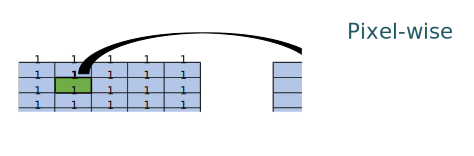
\includegraphics[height=2.2cm]{../figures/pixel_wise_algorithm}
    \hfill
    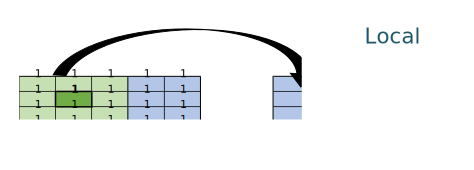
\includegraphics[height=2.2cm]{../figures/local_algorithm} \\
    \vspace{-0.05cm}
    \flushleft
    \hspace{0.53cm}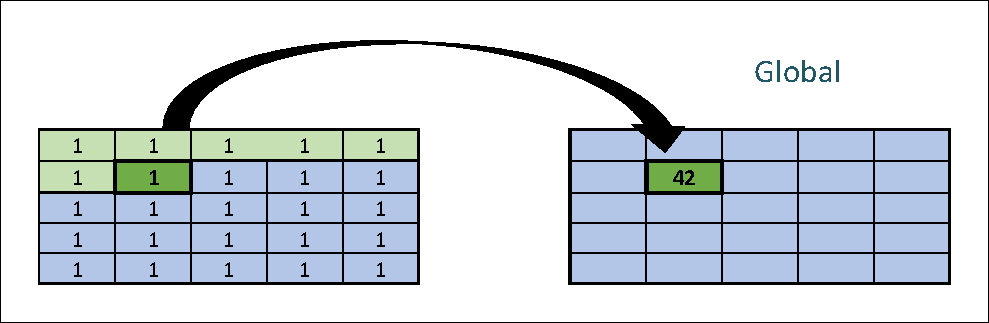
\includegraphics[height=2.2cm]{../figures/global_algorithm}
    \hfill
  \end{figure}
  \begin{textblock*}{5.5cm}(9.2cm,7.3cm)
    From those families emerge several concepts.
  \end{textblock*}
  \pdfcomment[icon=Note]{Nous avons identifié 3 familles d'algorithme de traitement d'image :}
  \pdfcomment[icon=Note]{- les algorithmes pixel par pixel}
  \pdfcomment[icon=Note]{- les algorithmes locaux (fênetre locale autour du pixel considéré, voisinage, élément structurant)}
  \pdfcomment[icon=Note]{- les algorithmes globaux (besoin de plusieurs passes dans plusieurs sens (avant, arrière, zigzag), besoin de piocher les pixels avec une logique autre qu'un parcours linéaire, besoin de considérer les valeurs tous les pixels de 1 à n-1 pour calculer n, etc.)}
  \pnote{
    Nous avons identifié 3 familles d'algorithme de traitement d'image :
    - les algorithmes pixel par pixel
    - les algorithmes locaux (fênetre locale autour du pixel considéré, voisinage, élément structurant)
    - les algorithmes globaux (besoin de plusieurs passes dans plusieurs sens (avant, arrière, zigzag), besoin de piocher les pixels avec une logique autre qu'un parcours linéaire, besoin de considérer les valeurs tous les pixels de 1 à n-1 pour calculer n, etc.)
  }
\end{frame}

\subsection{Concepts for Image Processing algorithms}

\begin{frame}[fragile]{Our Concepts for Image Processing: fundamentals}
  Fundamental concepts are necessary to be able to do basic manipulations over an image.
  \begin{itemize}
    \item Value, Point, Pixels: \GRAYOUT{represent the trivial building blocks of an image.}
    \item Domain: \GRAYOUT{represent the set of points valid for a given image (definition domain).}
    \item Image: \GRAYOUT{represent the algebraic relation \(y = f(x)\) where \(y\) is a value generated by the image \(f\) for
            the input (point) \(x\).}
    \item An image can also store a value, as in \(f(x) = y\).
  \end{itemize}
  Concepts interact with each other's through \hl{composition} and \hl{refinement} (close to inheritance).
  \pdfcomment[icon=Note]{De ces algorithmes émergent donc les concepts fondamentaux suivants:}
  \pdfcomment[icon=Note]{- Pixel, couple point -> valeur}
  \pdfcomment[icon=Note]{- Domaine de définition d'une image, au sens algébrique du terme}
  \pdfcomment[icon=Note]{- Image, représente la relation algébrique y = f(x) et f(x) = y pour les images inscriptibles}
  \pdfcomment[icon=Note]{   }
  \pdfcomment[icon=Note]{Relation entres concepts : composition et raffinage (proche de l'héritage pour le polymorphisme d'inclusion)}
  \pnote{
    De ces algorithmes émergent donc les concepts fondamentaux suivants:
    - Pixel, couple point -> valeur
    - Domaine de définition d'une image, au sens algébrique du terme
    - Image, représente la relation algébrique y = f(x) et f(x) = y pour les images inscriptibles

    Relation entres concepts : composition et raffinage (proche de l'héritage pour le polymorphisme d'inclusion)
  }
\end{frame}

\begin{frame}[fragile]{Our Concepts for Image Processing: fundamentals}
  The basic use case of a pixel-wise algorithm on an image is illustrated by the following code:
  \begin{minted}{C++}
    for (auto pnt : ima.domain()) // traverse image
      ima(pnt) = 42;              // Set the image's value at pnt
    
    // OR

    for (auto pix : ima.pixels()) // 0 cost abstraction
      pix.val() = 42;             // Set the pixel's value
      pix.val() = 42;             // Set the pixel's value
  \end{minted}
  \pdfcomment[icon=Note]{Voici le pattern comportemental de base pour une image.}
  \pdfcomment[icon=Note]{Nous voulons la parcourir de manière linéaire et assigner une valeur au pixel.}
  \pdfcomment[icon=Note]{   }
  \pdfcomment[icon=Note]{parcours des points -> marche mais n'est pas optimisé}
  \pdfcomment[icon=Note]{parcours des pixels -> marche et est optimisé car nous renvons des itérateurs dont l'abstration permet des optimisations similaire à du code C compréhensibles par le compilateur (pour de la vectorisation)}
  \pnote{
    Voici le pattern comportemental de base pour une image.
    Nous voulons la parcourir de manière linéaire et assigner une valeur au pixel.

    parcours des points -> marche mais n'est pas optimisé
    parcours des pixels -> marche et est optimisé car nous renvons des itérateurs dont l'abstration permet des optimisations similaire à du code C compréhensibles par le compilateur (pour de la vectorisation)
  }
\end{frame}

\begin{frame}[fragile]{Our Concepts for Image Processing: Image concept}
  \centering
  \begin{figure}
    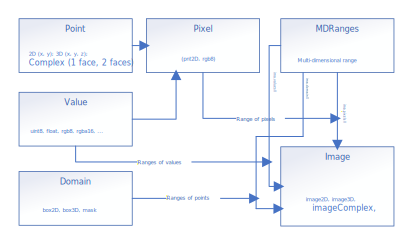
\includegraphics[width=0.9\textwidth]{../figures/concepts/image}
  \end{figure}
  \pdfcomment[icon=Note]{Cela donne donc la hiérarchie suivante:}
  \pdfcomment[icon=Note]{- concept pixel composé des concepts points/valeurs}
  \pdfcomment[icon=Note]{- concept mdrange modélise une range de point/valeurs/pixels}
  \pdfcomment[icon=Note]{- domaine de définition de l'image}
  \pdfcomment[icon=Note]{- ima.values() -> parcours de toutes les valeurs de l'image}
  \pdfcomment[icon=Note]{- ima.domain() -> parcours tous les points de l'image}
  \pdfcomment[icon=Note]{- ima.pixels() -> parcours tous les pixels de l'image}
  \pnote{
    Cela donne donc la hiérarchie suivante:
    - concept pixel composé des concepts points/valeurs
    - concept mdrange modélise une range de point/valeurs/pixels
    - domaine de définition de l'image
    - ima.values() -> parcours de toutes les valeurs de l'image
    - ima.domain() -> parcours tous les points de l'image
    - ima.pixels() -> parcours tous les pixels de l'image
  }
\end{frame}

\begin{frame}[fragile]{Our Concepts for Image Processing: Advanced Image concept}
  \begin{itemize}
    \item IndexableImage: access an image via indexes. \GRAYOUT{Needed for sorting pixels.}
          \begin{minted}{C++}
    auto v = ima[k];                                    // Access value from an index
    \end{minted}
    \item AccessibleImage: accessing image's value through points (seen above)
    \item BidirectionalImage: traversing image forward and backward \GRAYOUT{(such as Chamfer distance transform}.
          \begin{minted}{C++}
    for(auto pix : ima.pixels())                        // Forward pass
      pix.val() = /* ... */;
    for(auto pix : reversed(ima.pixels()))              // Backward pass
      pix.val() = /* ... */;
    \end{minted}
    \item RawImage: direct interface for accessing the image's data buffer. \GRAYOUT{Interface for experts.}
  \end{itemize}
  \pdfcomment[icon=Note]{Les images possèdent certaines propriétés qui peuvent être utilisé à des fins de caractérisation, discrimination (contraintes des algorithmes) ou encore d'optimisation}
  \pdfcomment[icon=Note]{   }
  \pdfcomment[icon=Note]{Indexable permet un parcours de toutes les valeurs lorsqu'on connait la dimension de l'image. Nécessaire pour trier les pixels.}
  \pdfcomment[icon=Note]{   }
  \pdfcomment[icon=Note]{Accessible permet d'accèder à une valeur via un point (vu plus haut)}
  \pdfcomment[icon=Note]{   }
  \pdfcomment[icon=Note]{Bidirectionnelle permet de traverser l'image en sens inverse, nécessaire pour certains algorithmes comme la transformé en distance de Chamfrain}
  \pdfcomment[icon=Note]{   }
  \pdfcomment[icon=Note]{Image brute permet un accès direct au buffer de donnée pour les utilisateurs expert, souhaitant par exemple couper leur image en tuiles pour l;es envoyer sur GPU.}
  \pnote{
    Les images possèdent certaines propriétés qui peuvent être utilisé à des fins de caractérisation, discrimination (contraintes des algorithmes) ou encore d'optimisation

    Indexable permet un parcours de toutes les valeurs lorsqu'on connait la dimension de l'image. Nécessaire pour trier les pixels.

    Accessible permet d'accèder à une valeur via un point (vu plus haut)

    Bidirectionnelle permet de traverser l'image en sens inverse, nécessaire pour certains algorithmes comme la transformé en distance de Chamfrain

    Image brute permet un accès direct au buffer de donnée pour les utilisateurs expert, souhaitant par exemple couper leur image en tuiles pour l;es envoyer sur GPU.
  }
\end{frame}

\begin{frame}[fragile]{Our Concepts for Image Processing: Advanced Image concept}
  \begin{figure}
    \flushleft
    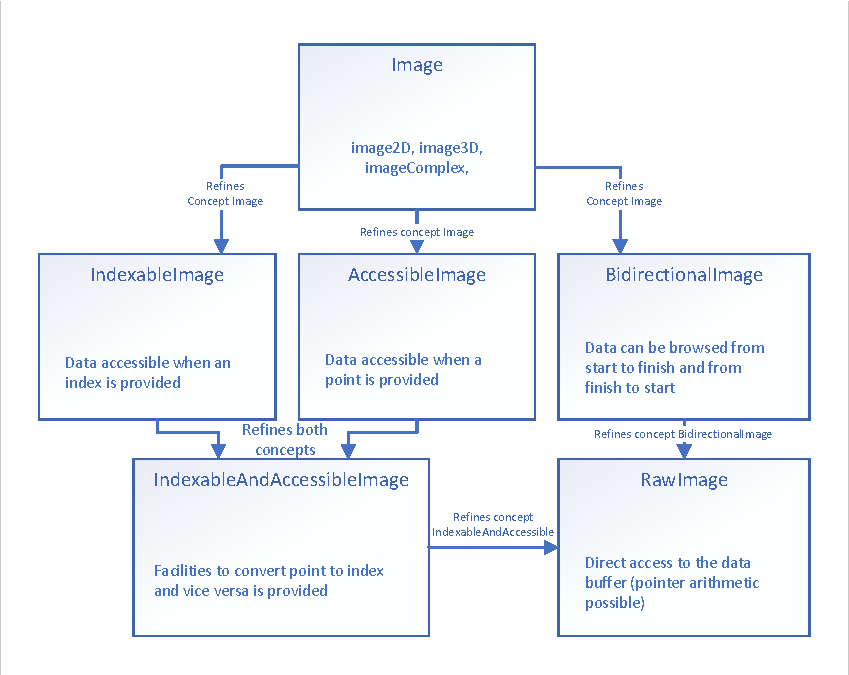
\includegraphics[width=0.65\textwidth]{../figures/concepts/images_all_rework}
  \end{figure}
  \begin{textblock*}{4cm}(11cm,5cm)
    \Large\textbf{\(+\) Writability}
  \end{textblock*}
  \pdfcomment[icon=Note]{Cela engendre donc cette nouvelle hiérarchie de concepts.}
  \pdfcomment[icon=Note]{   }
  \pdfcomment[icon=Note]{Ici nous avons 3 niveaux :}
  \pdfcomment[icon=Note]{- premier est concept image vu plus haut}
  \pdfcomment[icon=Note]{- second sont les concepts Indexable, Accessible et Bidirectionnelle qui rafinent le premier}
  \pdfcomment[icon=Note]{- 2.5 : concept spécial Indexable + Accessible pour faire des correspondances entre les indexes et les points}
  \pdfcomment[icon=Note]{- 3 image brute. En effet, lorsqu'on a accès au buffer de données, on peut faire tout ce qui est marqué plus haut.}
  \pdfcomment[icon=Note]{   }
  \pdfcomment[icon=Note]{Et SURTOUT PENDANT INSCRIPTIBLE DE CES CONCEPTS}
  \pdfcomment[icon=Note]{En effet, pour chaque propriété il est possible d'écrire des valeurs dans l'image.}
  \pnote{
    Cela engendre donc cette nouvelle hiérarchie de concepts.

    Ici nous avons 3 niveaux :
    - premier est concept image vu plus haut
    - second sont les concepts Indexable, Accessible et Bidirectionnelle qui rafinent le premier
    - 2.5 : concept spécial Indexable + Accessible pour faire des correspondances entre les indexes et les points
    - 3 image brute. En effet, lorsqu'on a accès au buffer de données, on peut faire tout ce qui est marqué plus haut.

    Et SURTOUT PENDANT INSCRIPTIBLE DE CES CONCEPTS
    En effet, pour chaque propriété il est possible d'écrire des valeurs dans l'image.
  }
\end{frame}


\begin{frame}[fragile]{Our Concepts for Image Processing: Local algorithms}
  \begin{itemize}
    \item Support for structuring elements (disc, rectangle, sphere, cube, etc.)
    \item Support retrieving neighboring pixels via the structuring element.
  \end{itemize}
  Typical usage in local algorithms:

  \begin{minted}{C++}
      auto se = se::disc(.radius=3); // get a structuring element
      for(auto pnt : ima.domain())   // traverse image's points
        for(auto nbp : se(pnt))      // traverse neighboring points
          // nbp is a range of points

      // OR

      for(auto pix : ima.pixels())   // 0 cost abstraction
        for(auto nbx : se(pix))      // traverse neighboring pixels
          // nbx is a range of pixels
  \end{minted}
  \pdfcomment[icon=Note]{Maintenant que nous avons tout le nécessaire pour les algorithmes locaux, il faut étendre un peu notre environnement pour supporter les algorithmes locaux.}
  \pdfcomment[icon=Note]{   }
  \pdfcomment[icon=Note]{Pattern comportemental typique : récupérer tous les points/pixels du voisinages et itérer dessus pour les traiter.}
  \pnote{
    Maintenant que nous avons tout le nécessaire pour les algorithmes locaux, il faut étendre un peu notre environnement pour supporter les algorithmes locaux.

    Pattern comportemental typique : récupérer tous les points/pixels du voisinages et itérer dessus pour les traiter.
  }
\end{frame}

\begin{frame}[fragile]{Our Concepts for Image Processing: Local algorithms}
  \centering
  \begin{figure}
    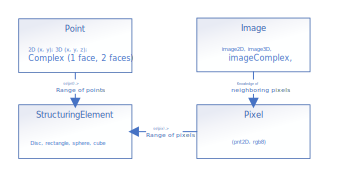
\includegraphics[width=0.7\textwidth]{../figures/concepts/se_extension_rework}
  \end{figure}
  \pdfcomment[icon=Note]{Cela donne donc lieu à la hiérchie de concepts suivante.}
  \pdfcomment[icon=Note]{   }
  \pdfcomment[icon=Note]{Ici se(pix) renvoie une range de pixels. se(pnt) renvoie une range de points.}
  \pdfcomment[icon=Note]{Et Pixel connait l'image car il peut donner ses pixels voisins.}
  \pnote{
    Cela donne donc lieu à la hiérchie de concepts suivante.

    Ici se(pix) renvoie une range de pixels. se(pnt) renvoie une range de points.
    Et Pixel connait l'image car il peut donner ses pixels voisins.
  }
\end{frame}

\subsection{Algorithms canvas}

\begin{frame}[fragile]{0-overhead for designed abstraction}
  % FIXME: retravailler transition
  \begin{itemize}
    \item We designed abstraction around those concepts that enables 0-overhead when they are used properly.
    \item For the majority of cases the default code will be the most efficient.
    \item It is possible to dispatch (dynamically of statically) to algorithms specialization for the remaining edge
          cases for maximum efficiency.
  \end{itemize}
  \begin{columns}[T,onlytextwidth]
    \column{0.50\textwidth}
    \begin{minted}{C++}
      template <Image Img, StructuringElement SE>
      auto dilate(Img img, SE se) {
        if (se.is_decomposable()) {
          lst_small_se = se.decompose();
          for (auto small_se : lst_small_se)
            // Recursive call
            img = dilate(img, small_se);
          return img;
        }
          \end{minted}

    \column{0.50\textwidth}
    \begin{minted}{C++}
        else if (is_pediodic_line(se))
            // Van Herk's algorithm
          return fast_dilate1d(img, se);
        else
            // Classic algorithm
          return dilate_normal(img, se);
      }
      \end{minted}
  \end{columns}

  %\column{0.40\textwidth}
  %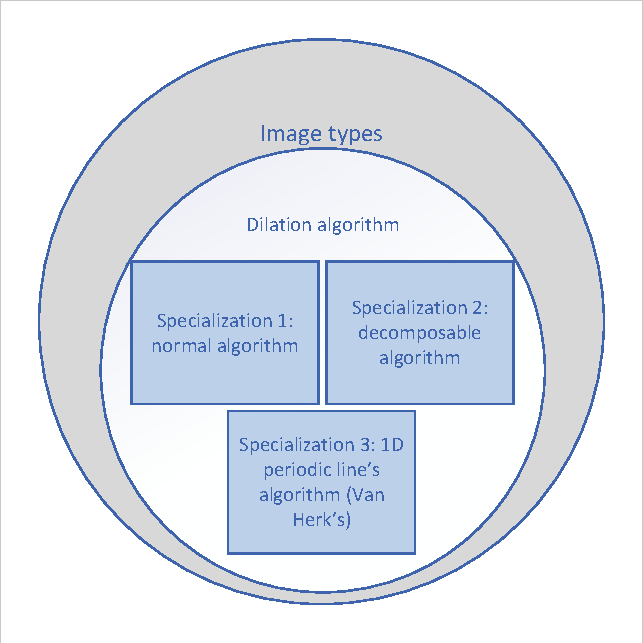
\includegraphics[width=0.99\textwidth]{../figures/dilation_specialization_diagram}
  \pdfcomment[icon=Note]{Nous ayons designé un environnement de concepts dont le but et d'avoir un surcoût de 0 à l'exécution et d'être optimisé par le compilateur.}
  \pdfcomment[icon=Note]{   }
  \pdfcomment[icon=Note]{Dans l'imense majorité des cas, le code par dafaut sera donc le plus performant.}
  \pdfcomment[icon=Note]{   }
  \pdfcomment[icon=Note]{Dans de rare cas, cependant, il est possible d'aller encore plus vite en exploitant certaines propriétés liées à l'image ou aux structures auxiliaires utilisées dans ces algorithmes.}
  \pdfcomment[icon=Note]{   }
  \pdfcomment[icon=Note]{Par ex, dilatation ici, on utilise la propriété relative à la decomposabilité et à la périodicité pour améliorer les performance.}
  \pdfcomment[icon=Note]{   }
  \pdfcomment[icon=Note]{Ces propriété peuvent être dynamic ou statique (transformer if par if constexpr).}
  \pnote{
    Nous ayons designé un environnement de concepts dont le but et d'avoir un surcoût de 0 à l'exécution et d'être optimisé par le compilateur.

    Dans l'imense majorité des cas, le code par dafaut sera donc le plus performant.

    Dans de rare cas, cependant, il est possible d'aller encore plus vite en exploitant certaines propriétés liées à l'image ou aux structures auxiliaires utilisées dans ces algorithmes.

    Par ex, dilatation ici, on utilise la propriété relative à la decomposabilité et à la périodicité pour améliorer les performance.

    Ces propriété peuvent être dynamic ou statique (transformer if par if constexpr).
  }
\end{frame}

\begin{frame}[fragile]{Taxonomy for Image Processing: Canvas for Dilation \& Erosion}
  Dilation and Erosion have the same shape:
  \begin{columns}[T,onlytextwidth]
    \column{0.50\textwidth}
    \includegraphics[width=0.7\textwidth]{../figures/dilation_code_rework}

    \column{0.50\textwidth}
    \includegraphics[width=0.7\textwidth]{../figures/erosion_code_rework}
  \end{columns}
  \bigskip
  They can be rewritten in a common canvas:
  \begin{columns}[T,onlytextwidth]
    \column{0.50\textwidth}
    \includegraphics[width=0.7\textwidth]{../figures/local_op_code_rework}

    \column{0.50\textwidth}
    \includegraphics[width=0.9\textwidth]{../figures/local_op_dilation_code_rework}
    \includegraphics[width=0.9\textwidth]{../figures/local_op_erosion_code_rework}
  \end{columns}
  \pdfcomment[icon=Note]{En faisant la taxonomie liée au algorithmes locaux, nous nous sommes aperçu que les algorithmes avaient la même forme computationnelle.}
  \pdfcomment[icon=Note]{   }
  \pdfcomment[icon=Note]{Cela veut dire que nous pouvons factoriser le schéma algorithmique en meta-algorithmes que l'on appelle les canvas d'algorithme.}
  \pdfcomment[icon=Note]{   }
  \pdfcomment[icon=Note]{Par exemple ici dilatation erosion -> min/max, réécriture en passant l'opérateur en paramètre.}
  \pdfcomment[icon=Note]{   }
  \pdfcomment[icon=Note]{Canvas d'algorithme local simplifié.}
  \pnote{
    En faisant la taxonomie liée au algorithmes locaux, nous nous sommes aperçu que les algorithmes avaient la même forme computationnelle.

    Cela veut dire que nous pouvons factoriser le schéma algorithmique en meta-algorithmes que l'on appelle les canvas d'algorithme.

    Par exemple ici dilatation erosion -> min/max, réécriture en passant l'opérateur en paramètre.

    Canvas d'algorithme local simplifié.
  }
\end{frame}

\begin{frame}[fragile]{Taxonomy for Image Processing: Algorithms over-generalization}
  \begin{itemize}
    \item Algorithms can have the same computational shape.
    \item When this shape is known, an algorithm canvas can be written (meta-algorithm)
    \item This canvas shifts the algorithm implementation into a descriptive paradigm.
    \item This canvas allows reusing code easily.
    \item This canvas allows the maintainer to factorize optimizations (GPU offloading, etc.)
  \end{itemize}
  \pdfcomment[icon=Note]{Possible opportinutés d'optimisations implémenté une fois et factorisé pour tous les algorithmes.}
  \pdfcomment[icon=Note]{   }
  \pdfcomment[icon=Note]{En revanche on passe d'un paradigme d'implémentation procédurial de nos algorithmes à un paradigme de description de nos algorithmes (pour le canvas), ce qui peut rendre l'implémentation moins lisible, surtout lorsqu'il y a des callbacks.}
  \pnote{
    Possible opportinutés d'optimisations implémenté une fois et factorisé pour tous les algorithmes.

    En revanche on passe d'un paradigme d'implémentation procédurial de nos algorithmes à un paradigme de description de nos algorithmes (pour le canvas), ce qui peut rendre l'implémentation moins lisible, surtout lorsqu'il y a des callbacks.
  }
\end{frame}

%
%
%
\section[Views for image processing (contribution)]{Views for image processing (contribution)}

\begin{frame}{Outline}
  \setbeamertemplate{section in toc}[sections numbered]
  \vspace{0.2cm}
  \small%\singlespacing
  \tableofcontents[currentsection]
  \pdfcomment[icon=Note]{Maintenant que nous avons designé un environnement complet de concepts pour faire de la généricité contrainte en traitement d'image, utilisons le pour créer des nouveaux type d'image : les vues, qui utilisent ces concepts (propriétés) pour abstraires des algorithmes, tout en respectant le principe d'abstration à coût 0.}
  \pdfcomment[icon=Note]{   }
  \pdfcomment[icon=Note]{--> 30min <--}
  \pnote{
    Maintenant que nous avons designé un environnement complet de concepts pour faire de la généricité contrainte en traitement d'image, utilisons le pour créer des nouveaux type d'image : les vues, qui utilisent ces concepts (propriétés) pour abstraires des algorithmes, tout en respectant le principe d'abstration à coût 0.

    --> 30min <--
  }
\end{frame}

\subsection{Genesis of a new abstraction layer: Views}

\begin{frame}[fragile]{Views for Image Processing}
  \begin{alertblock}{View definition}
    A view \hl{is an \emph{image}} which embarks an algorithm and features properties. They are inspired from Milena's
    morphers~\footnote{Levillain et al., Milena: Write generic morphological algorithms once, run on many kinds of
      images. ISMM 2009.} and STL ranges~\footnote{Niebler et al., Ranges for the standard library: Revision 1. ISO WG21,
      2014.}. We published our take in~\footnote{Roynard et al., A modern C++ point of View of programming in image
      processing. ACM SIGPLAN GPCE, 2022.}.

    %In Pylene, \hl{a View \textbf{IS} an Image} and \hl{all Image are lightweight} objects (cheap-to-copy). Images have
    %\hl{value semantic} and copies perform \emph{shallow-copies} with a shared data buffer by default.
  \end{alertblock}
  \begin{center}\textbf{Views can replace pixel-wise algorithms.}\end{center}
  \pdfcomment[icon=Note]{Les vues sont des images.}
  \pdfcomment[icon=Note]{   }
  \pdfcomment[icon=Note]{Elles emarquent des algorithmes pixel par pixel en leur sein.}
  \pdfcomment[icon=Note]{   }
  \pdfcomment[icon=Note]{Elles sont inspirées des morphers de Milena et des ranges de la STL.}
  \pdfcomment[icon=Note]{   }
  \pdfcomment[icon=Note]{Les vues ont vocation à complétement remplacer les algorithmes pixel par pixel.}
  \pnote{
    Les vues sont des images.

    Elles emarquent des algorithmes pixel par pixel en leur sein.

    Elles sont inspirées des morphers de Milena et des ranges de la STL.

    Les vues ont vocation à complétement remplacer les algorithmes pixel par pixel.
  }
\end{frame}

% levillain.2009.ismm
% Levillain, R., Géraud, T., & Najman, L. (2009). Milena: Write generic morphological algorithms once, run on many kinds
% of images. In M. H. F. Wilkinson & J. B. T. M. Roerdink (Eds.), Mathematical morphology and its application to signal
% and image processing — proceedings of the ninth international symposium on mathematical morphology (ismm) (pp.
% 295–306, Vol. 5720). Springer Berlin / Heidelberg. (Cit. on p. 38).

% niebler.2014.ranges
% Eric Niebler, A. S., Sean Parent. (2014). Ranges for the standard library: Revision 1.
% https://ericniebler.github.io/std/wg21/D4128.html (cit. on p. 38).

% roynard.2022.gpce
% Roynard, M., Carlinet, E., & Géraud, T. (2022). A modern C++ point of View of programming in image processing.
% Proceedings of the 21st ACM SIGPLAN International Conference on Generative Programming: Concepts and Experiences (GPCE
% ’22), December 06–07, 2022, Auckland, New Zealand. https://doi.org/10.1145/3564719.3568692 (cit. on pp. 38, 54).

\begin{frame}[fragile]{View properties}
  Views feature interesting properties.
  \begin{columns}[T,onlytextwidth]
    \column{0.350\textwidth}
    They are:
    \begin{alertblock}{View properties}
      \begin{itemize}
        \item Cheap-to-copy (lightweight),
        \item Non-owning (shared semantic of the data buffer),
        \item Lazy evaluated,
        \item Composable.
      \end{itemize}
    \end{alertblock}

    \column{0.65\textwidth}
    \begin{figure}
      \begin{minipage}{\linewidth}
        \includegraphics[height=4cm]{../figures/transform_thresholding}
      \end{minipage}
      \caption{An image view performing a thresholding.}
      \label{fig.view.threshold}
    \end{figure}
  \end{columns}
  \pdfcomment[icon=Note]{Voici un exemple de vue pour effectuer une binarisation.}
  \pdfcomment[icon=Note]{   }
  \pdfcomment[icon=Note]{Cette vu contient 2 pointeurs (fonction + image de base)}
  \pdfcomment[icon=Note]{   }
  \pdfcomment[icon=Note]{Sémantique de partage du buffer de donné (pour éviter les violations mémoires)}
  \pdfcomment[icon=Note]{   }
  \pdfcomment[icon=Note]{Sémantique de copie superficielle}
  \pdfcomment[icon=Note]{   }
  \pdfcomment[icon=Note]{Evaluation paresseuse}
  \pdfcomment[icon=Note]{   }
  \pdfcomment[icon=Note]{Composables}
  \pnote{
    Voici un exemple de vue pour effectuer une binarisation.

    Cette vu contient 2 pointeurs (fonction + image de base)

    Sémantique de partage du buffer de donné (pour éviter les violations mémoires)

    Sémantique de copie superficielle

    Evaluation paresseuse

    Composables
  }
\end{frame}

\subsection{Raising abstraction level}

\begin{frame}[fragile]{Raising abstraction level}
  Views enable the Image Processing practitioner to rewrite the following alpha-blending algorithm at image level.
  \begin{minted}{C++}
  void blend_inplace(const uint8_t* ima1, uint8_t* ima2, float alpha,
  int width, int height, int stride1, int stride2) {
    for (int y = 0; y < height; ++y) {
      const uint8_t* iptr = ima1 + y * stride1;
      uint8_t* optr = ima2 + y * stride2;
      for (int x = 0; x < width; ++x)
        optr[x] = iptr[x] * alpha + optr[x] * (1-alpha);
    }
  }
  \end{minted}
  \begin{figure}
    \flushleft
    \includegraphics[width=0.7\textwidth]{../figures/alphablend}
  \end{figure}
  \begin{textblock*}{4.5cm}(11.5cm,3.2cm)
    \begin{minted}[highlightlines={8-9},highlightcolor=yellow!60!white]{C++}
// ROI overload
void blend_inplace(
  const uint8_t* ima1,
  uint8_t* ima2,
  float alpha, int width,
  int height, int stride1,
  int stride2,
  int width_b, int width_e
  int height_b, int height_e);
    \end{minted}
  \end{textblock*}
  \pdfcomment[icon=Note]{Par exemple algorithme alphablending.}
  \pdfcomment[icon=Note]{   }
  \pdfcomment[icon=Note]{Code C basique, double boucle, arithmétique de pointeurs, strides etc.}
  \pdfcomment[icon=Note]{   }
  \pdfcomment[icon=Note]{Si l'on veut n'opérer que dans une région spécifique (région d'intérêt), on devrait définir une nouvelle implémentation avec un prototype différents.}
  \pdfcomment[icon=Note]{   }
  \pdfcomment[icon=Note]{En revanche, avec les vues cet algorithme s'exprime très simplement. Et comme les vues sont composables (slide suivante)}
  \pnote{
    Par exemple algorithme alphablending.

    Code C basique, double boucle, arithmétique de pointeurs, strides etc.

    Si l'on veut n'opérer que dans une région spécifique (région d'intérêt), on devrait définir une nouvelle implémentation avec un prototype différents.

    En revanche, avec les vues cet algorithme s'exprime très simplement. Et comme les vues sont composables (slide suivante)
  }
\end{frame}

\begin{frame}[fragile]{Views for Image Processing: Raising abstraction level}
  \begin{alertblock}{Composable:}
    \begin{minted}{C++}
auto roi = /* ... */;
auto blend_roi = alphablend(view::clip(ima1, roi), view::clip(ima2, roi), 0.2);
auto blend_red = alphablend(view::red(ima1), view::red(ima2), 0.2);
    \end{minted}
  \end{alertblock}
  \begin{alertblock}{Lazy-evaluated, Non-owning}
    \vspace{0.2cm}
    \begin{columns}[T,onlytextwidth]
      \column{0.5\textwidth}
      \begin{tcolorbox}
        \begin{minted}{C++}
  auto alphablend =
  [](auto ima1, auto ima2, float alpha) {
    return alpha * ima1 +
                  (1 - alpha) * ima2;
  };
      \end{minted}
      \end{tcolorbox}

      \column{0.45\textwidth}
      \centering
      \begin{tcolorbox}
        \begin{figure}
          \includegraphics[width=0.68\textwidth]{../figures/view_ast2}
        \end{figure}
      \end{tcolorbox}

    \end{columns}
  \end{alertblock}
  \begin{alertblock}{Cheap-to-copy:}
    \begin{minted}{C++}
auto ima1, ima2 = /* ... */;
auto ima_blended = alphablend(ima1, ima2, 0.2);
    \end{minted}
  \end{alertblock}
  \pdfcomment[icon=Note]{On peut directement écrite vue clip de notre image puis la passer à notre algorithme.}
  \pdfcomment[icon=Note]{   }
  \pdfcomment[icon=Note]{Notre algorithme s'écrit très simplement}
  \pdfcomment[icon=Note]{Arbre de calcul généré et résolu lors du parcours de l'image (évaluation paresseuse)}
  \pdfcomment[icon=Note]{On prend ima1, ima2 par copie sans impact de performance}
  \pdfcomment[icon=Note]{On peut copier ima_blended sans dupliquer le buffer de donnée ni calculer l'entièreté de la transformation.}
  \pnote{
    On peut directement écrite vue clip de notre image puis la passer à notre algorithme.

    Notre algorithme s'écrit très simplement
    Arbre de calcul généré et résolu lors du parcours de l'image (évaluation paresseuse)
    On prend ima1, ima2 par copie sans impact de performance
    On peut copier ima_blended sans dupliquer le buffer de donnée ni calculer l'entièreté de la transformation.
  }
\end{frame}

% FIXME: discours vues similaire aux opérateurs de programmation fonctionnelle
\begin{frame}[fragile]{Overview of basic views}
  \begin{alertblock}{Domain-restrictive views: filter, clip, mask}
    \begin{columns}[T,onlytextwidth]
      \column{0.60\textwidth}
      \vspace{0.5cm}
      \includegraphics[width=0.9\textwidth]{../figures/views/mask_1}

      \column{0.40\textwidth}
      \vspace{0.5cm}
      \includegraphics[width=0.9\textwidth]{../figures/views/clip}
    \end{columns}
  \end{alertblock}

  \begin{alertblock}{Value-transforming view: transform, zip, cast, \(+\), \(\times\), etc.}
    \begin{columns}[T,onlytextwidth]
      \column{0.40\textwidth}
      \vspace{0.5cm}
      \includegraphics[width=0.9\textwidth]{../figures/views/transform_grey}

      \column{0.60\textwidth}
      \vspace{0.5cm}
      \includegraphics[width=0.9\textwidth]{../figures/views/zip}
    \end{columns}
  \end{alertblock}
  \pdfcomment[icon=Note]{Les vues sont très similaires aux opérateurs de base de la programmation fonctionnelle.}
  \pdfcomment[icon=Note]{   }
  \pdfcomment[icon=Note]{En effet on retrouve les vues qui vont restreindre le domaine de définition de nos images, filter, clip , mask.}
  \pdfcomment[icon=Note]{   }
  \pdfcomment[icon=Note]{On retrouve les vues qui vont transformer les valeurs de nos image zip, cast, +, * et transform}
  \pdfcomment[icon=Note]{   }
  \pdfcomment[icon=Note]{Transform va appliquer une fonction de transformation. Zip va assembler les valeurs en paire/triplet, très utile lorsqu'on itère sur une image d'entrée et une image de sortie en même temps.}
  \pnote{
    Les vues sont très similaires aux opérateurs de base de la programmation fonctionnelle.

    En effet on retrouve les vues qui vont restreindre le domaine de définition de nos images, filter, clip , mask.

    On retrouve les vues qui vont transformer les valeurs de nos image zip, cast, +, * et transform

    Transform va appliquer une fonction de transformation. Zip va assembler les valeurs en paire/triplet, très utile lorsqu'on itère sur une image d'entrée et une image de sortie en même temps.
  }
\end{frame}

\begin{frame}[fragile]{Property preservation (of concepts) through views}
  \centering
  \begin{figure}
    \includegraphics[width=0.9\textwidth]{../figures/view_property}
  \end{figure}
  \pdfcomment[icon=Note]{Les images sont des vues et en tant que tel il va être possible de vérifier quelles sont les propriétés vérifiables via des concepts qui sont conservées lorsque l'on compose ces images/vues.}
  \pdfcomment[icon=Note]{   }
  \pdfcomment[icon=Note]{Toutes les propriétés relatives au parcours et à l'accès aux valeurs sont conservés sauf celle relative au buffer de donnée.}
  \pdfcomment[icon=Note]{   }
  \pdfcomment[icon=Note]{En ce qui concerne l'inscriptibilité, il est intéressant de remarquer que la vue transform peut la conserver lorsque func est une projection.}
  \pdfcomment[icon=Note]{Ex triplet rgb -> rouge}
  \pdfcomment[icon=Note]{Mais triplet rgb -> gris, on ne retrouuve pas le triplet rgb en assignant une nouvelle valeure de niveau de gris. La recolorisation est un domaine de recherche à part entière.}
  \pnote{
    Les images sont des vues et en tant que tel il va être possible de vérifier quelles sont les propriétés vérifiables via des concepts qui sont conservées lorsque l'on compose ces images/vues.

    Toutes les propriétés relatives au parcours et à l'accès aux valeurs sont conservés sauf celle relative au buffer de donnée.

    En ce qui concerne l'inscriptibilité, il est intéressant de remarquer que la vue transform peut la conserver lorsque func est une projection.
    Ex triplet rgb -> rouge
    Mais triplet rgb -> gris, on ne retrouuve pas le triplet rgb en assignant une nouvelle valeure de niveau de gris. La recolorisation est un domaine de recherche à part entière.
  }
\end{frame}

\subsection{Background subtraction benchmark}

\begin{frame}[fragile]{Concrete application of Views: Background subtraction}
  \begin{figure}[htbp]
    \centering
    \begin{tabular}{cccc}
      Background                                                                        & Candidate & Result                     \\[5pt]
      \fbox{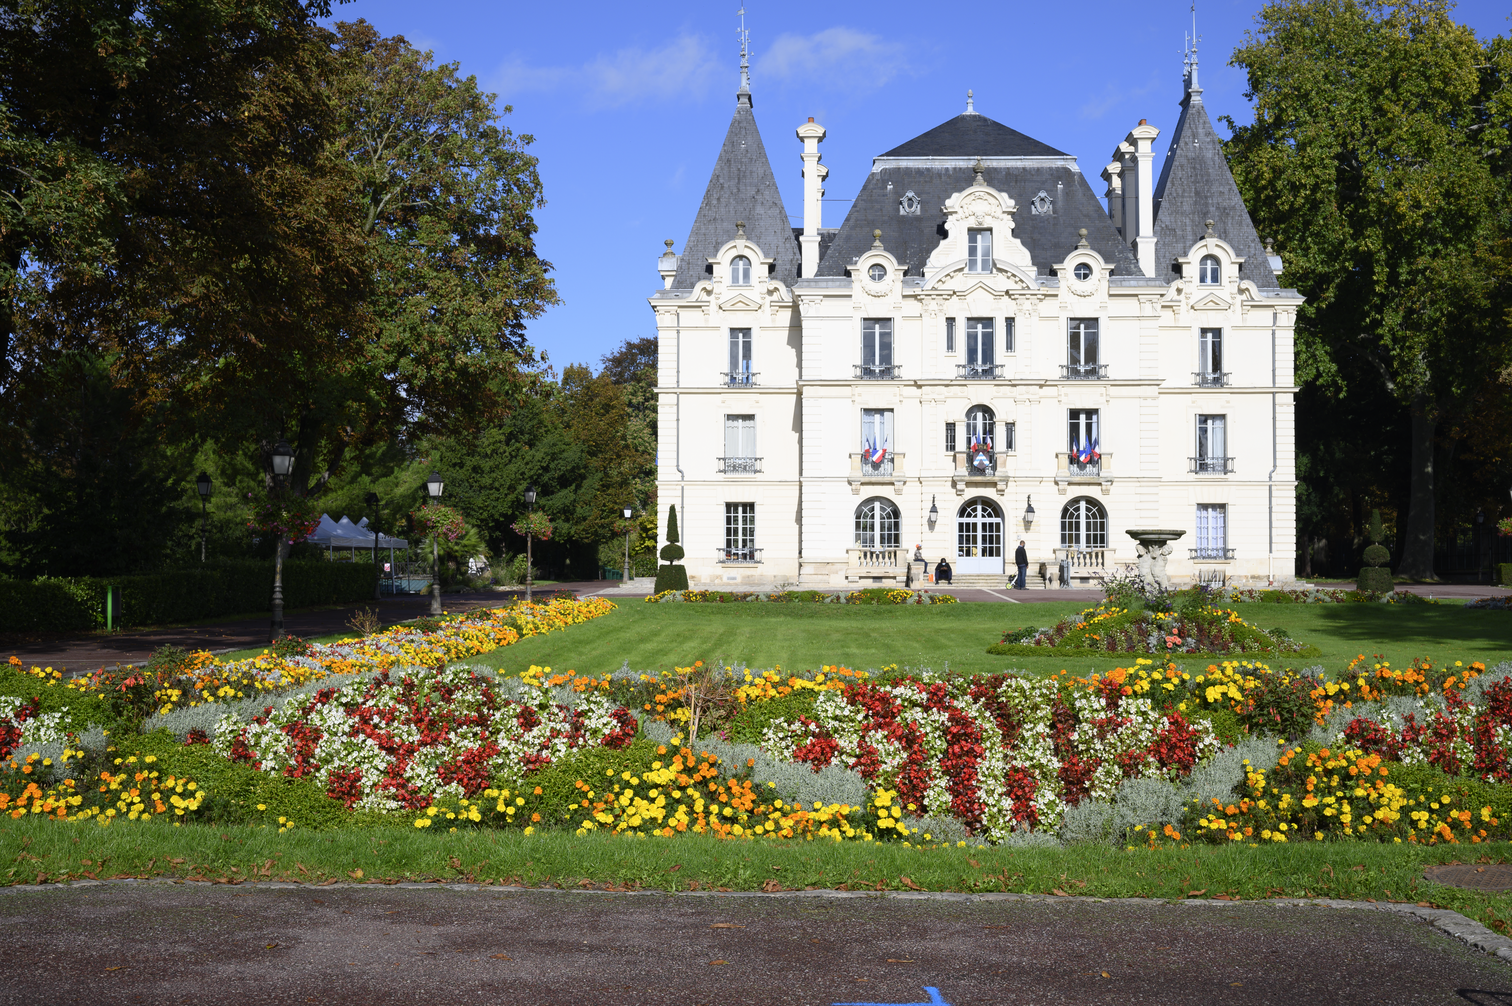
\includegraphics[width=.25\linewidth]{../assets/1512x1006/castle_bg.png}}   &
      \fbox{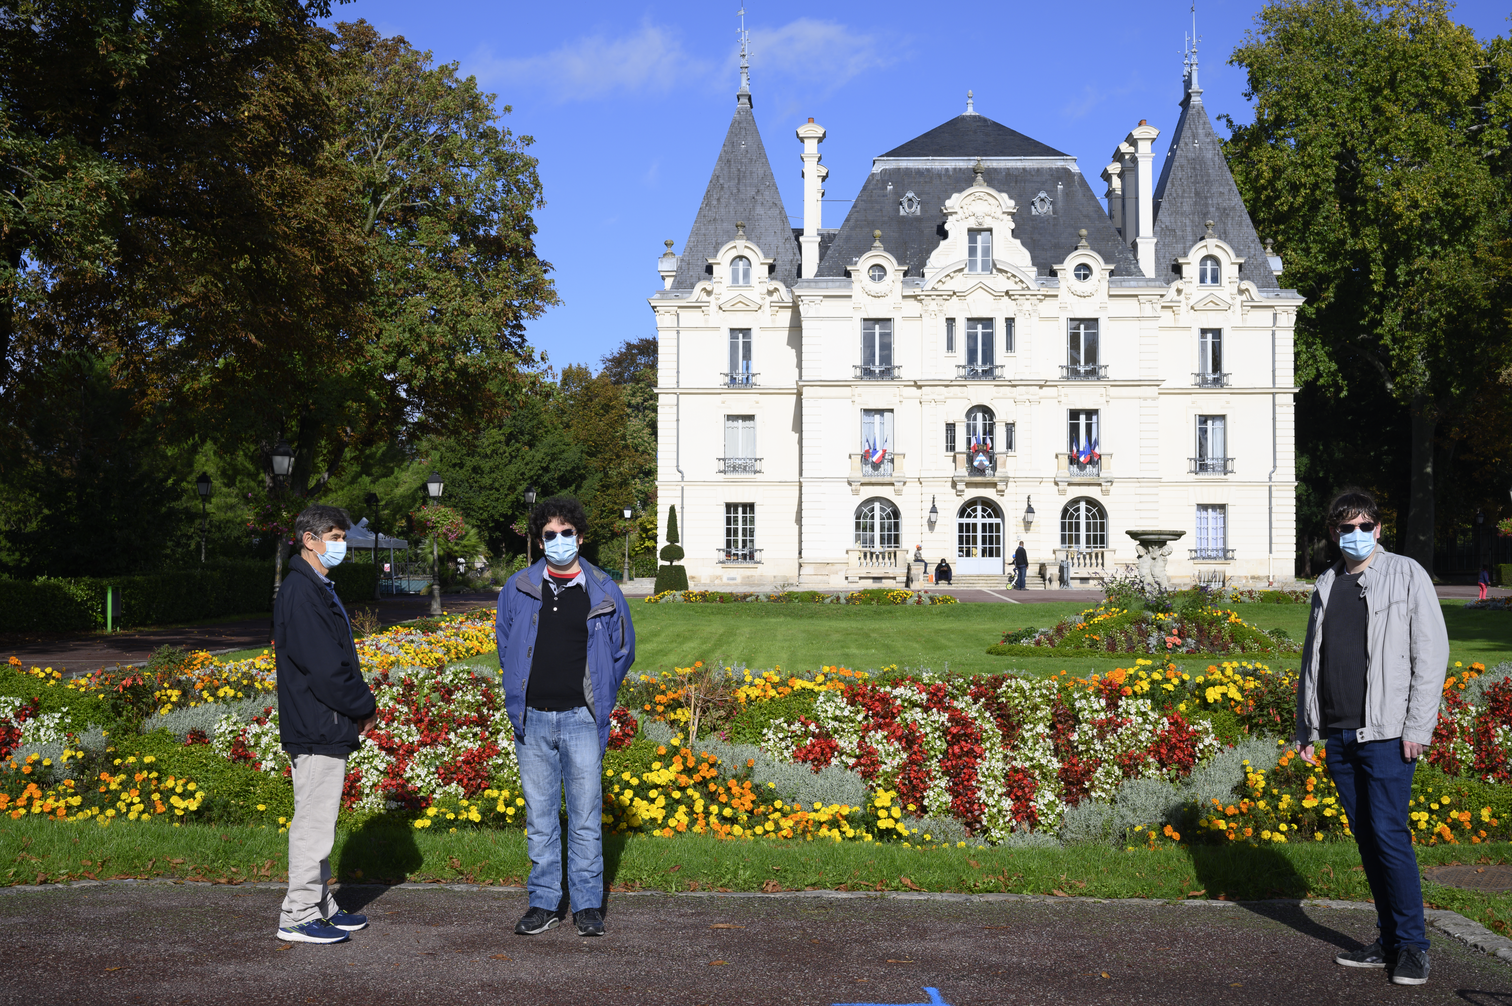
\includegraphics[width=.25\linewidth]{../assets/1512x1006/castle_fg_1.png}} &
      \fbox{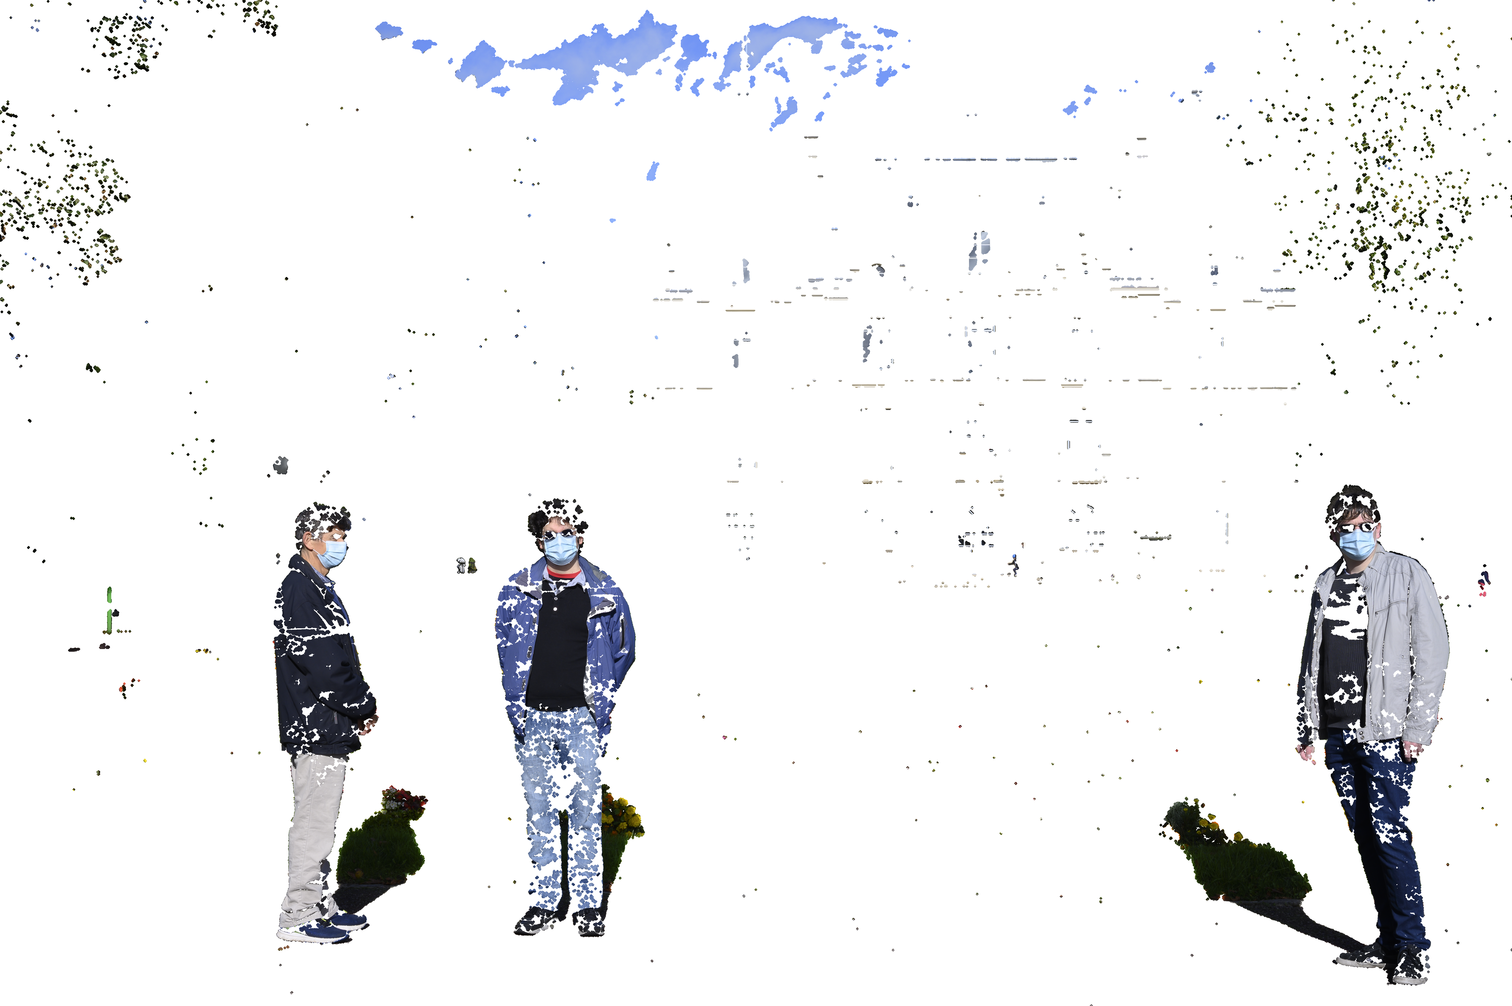
\includegraphics[width=.25\linewidth]{../assets/1512x1006/results_sig1_win5/castle/result_detected_castle_fg_1.png}} \\[5pt]
      \fbox{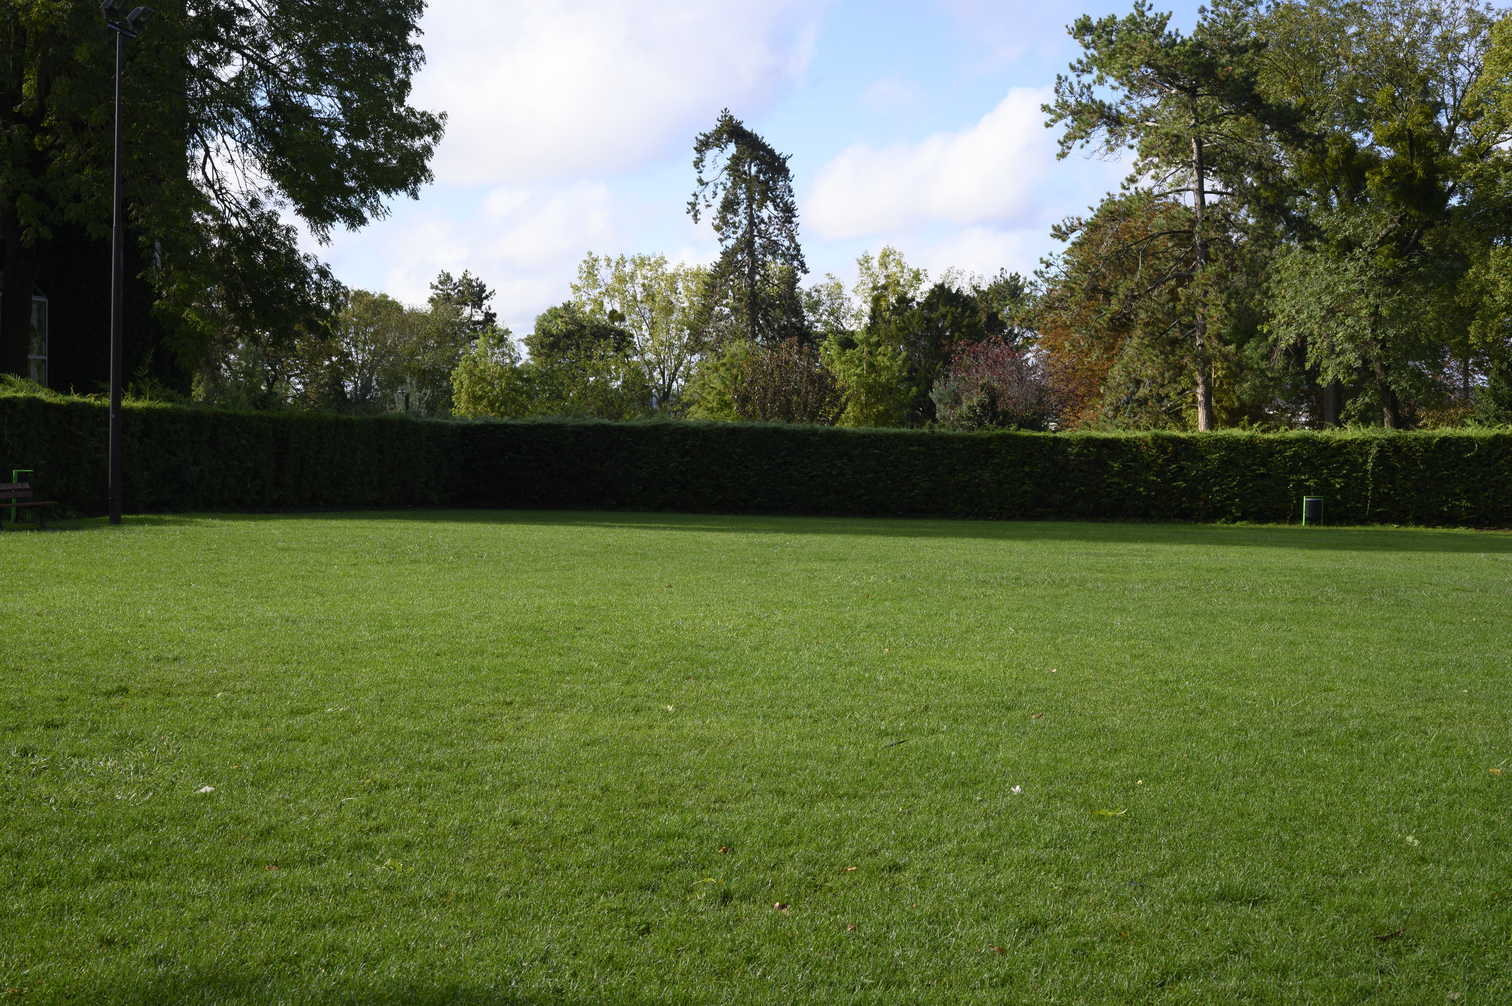
\includegraphics[width=.25\linewidth]{../assets/1512x1006/garden_bg.png}}   &
      \fbox{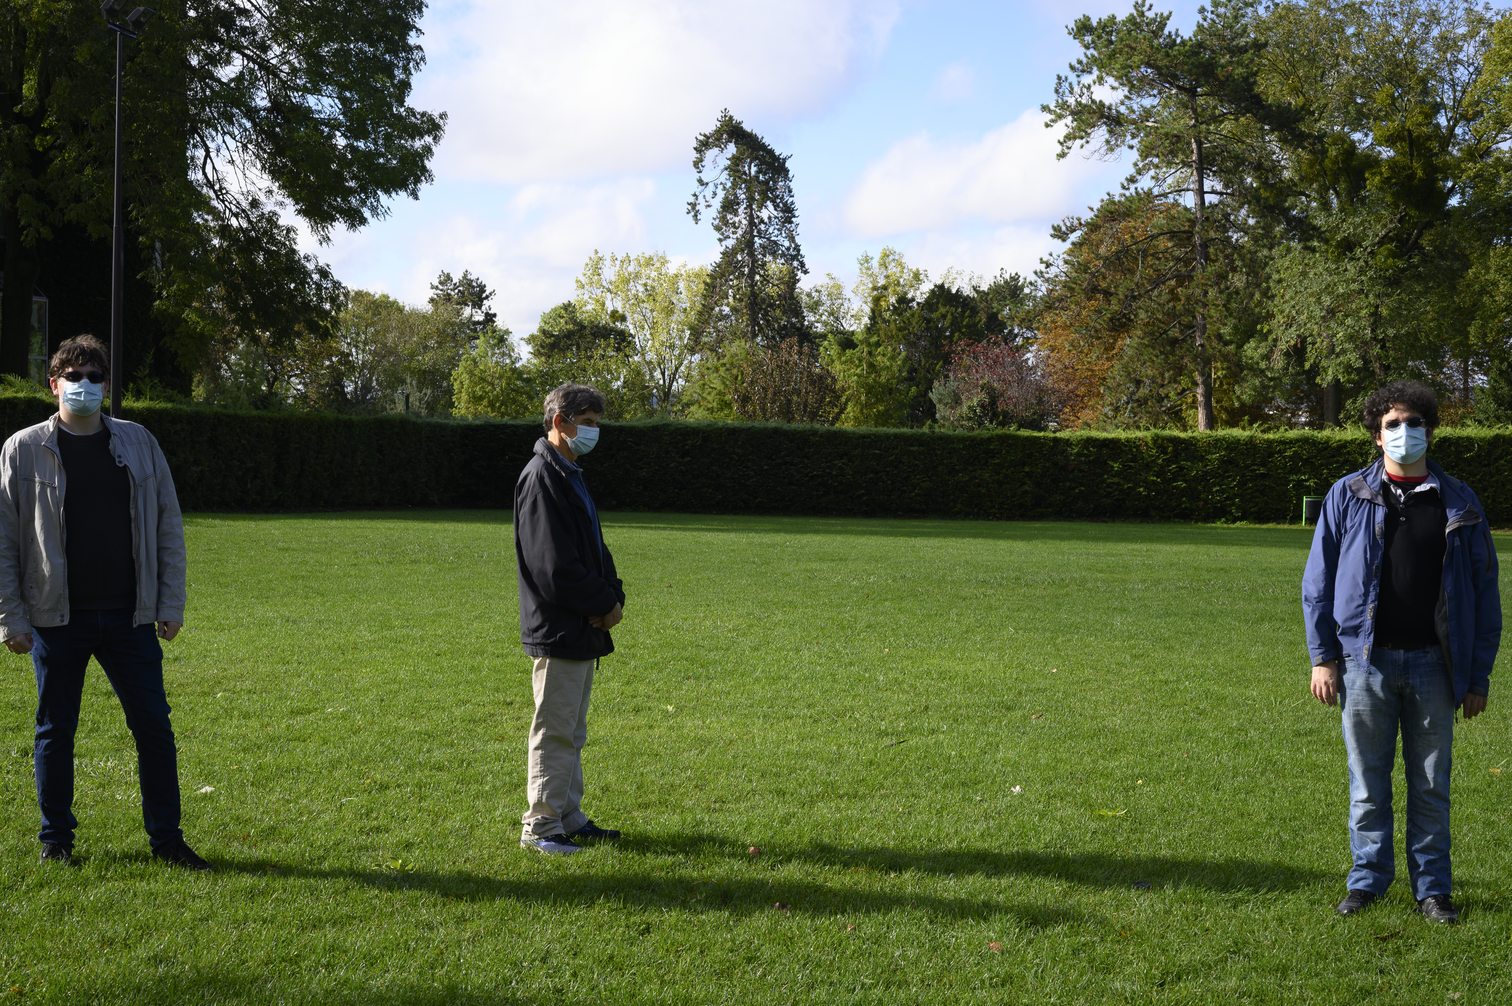
\includegraphics[width=.25\linewidth]{../assets/1512x1006/garden_fg_1.png}} &
      \fbox{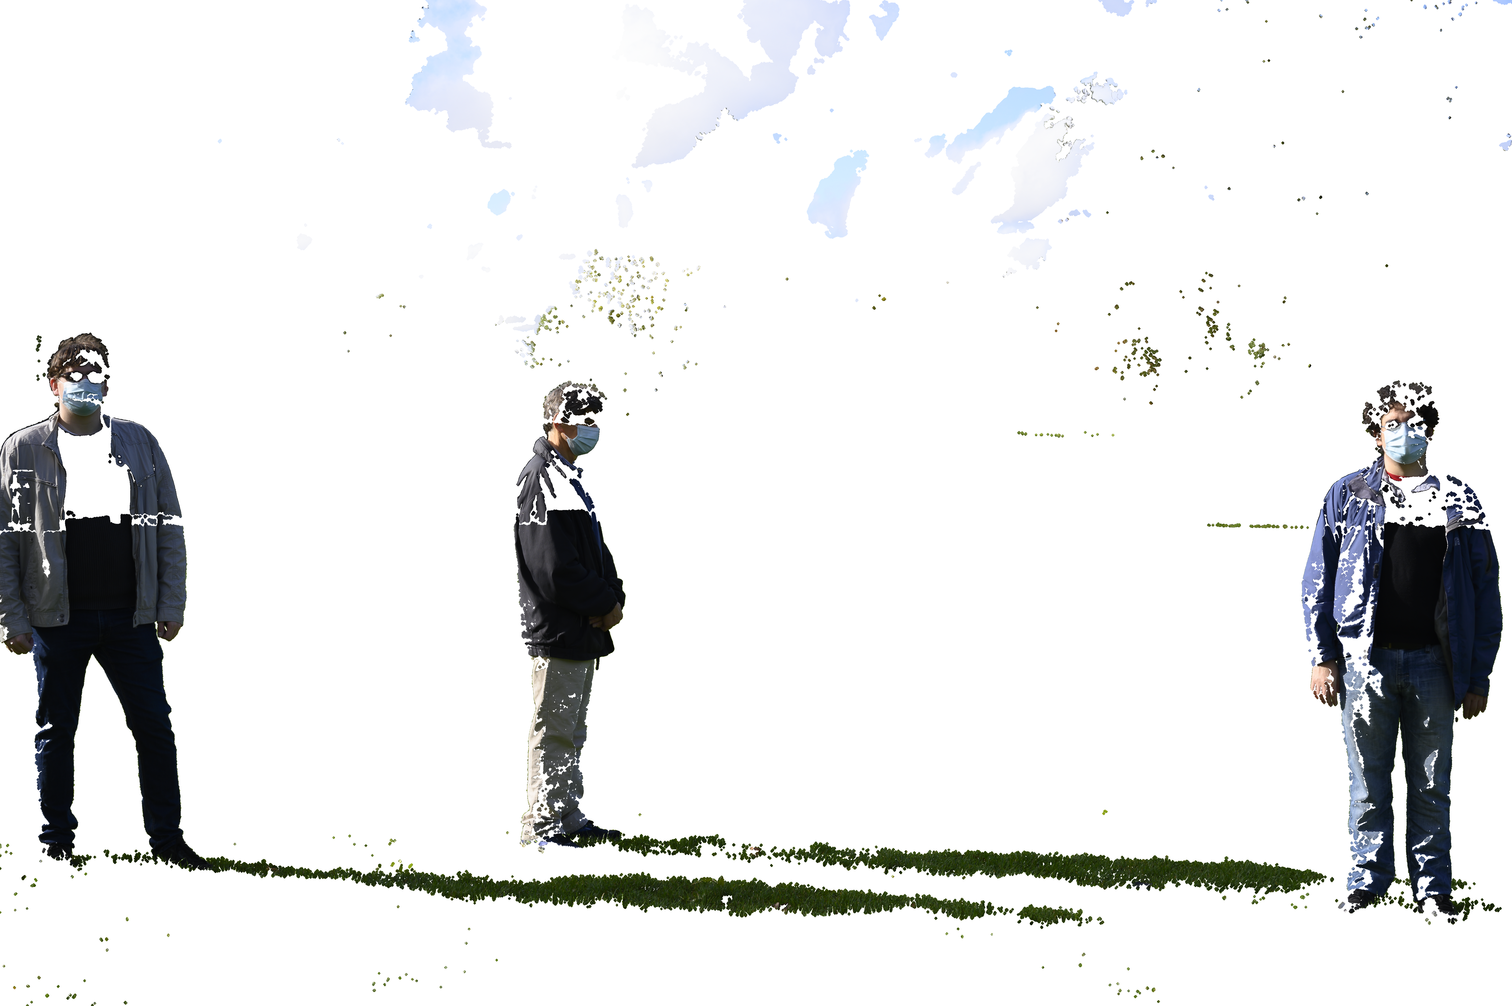
\includegraphics[width=.25\linewidth]{../assets/1512x1006/results_sig1_win5/garden/result_detected_garden_fg_1.png}}
    \end{tabular}

    \caption{Background detection: data set samples.}
    \label{fig:bg_sub.dataset_samples}
  \end{figure}
  \pdfcomment[icon=Note]{Nous avons vu en détail que les vues fonctionnait avec notre environement de concept et remplaçait les algorithmes pixel par pixel.}
  \pdfcomment[icon=Note]{   }
  \pdfcomment[icon=Note]{Il nous faut maintenant valider que cette abstraction est bel et bien 0-cost.}
  \pdfcomment[icon=Note]{   }
  \pdfcomment[icon=Note]{Voici l'algorithme de soustraction d'arrière plan que nous avons utiliser dans notre benchmark...}
  \pnote{
    Nous avons vu en détail que les vues fonctionnait avec notre environement de concept et remplaçait les algorithmes pixel par pixel.

    Il nous faut maintenant valider que cette abstraction est bel et bien 0-cost.

    Voici l'algorithme de soustraction d'arrière plan que nous avons utiliser dans notre benchmark...
  }
\end{frame}

\begin{frame}[fragile]{Background subtraction pipeline with algorithms}
  \begin{figure}[htbp]
    \centering
    \includegraphics[width=0.9\linewidth]{../figures/pipeline_bg_sub_comp_algo}
    \caption{Background subtraction pipeline using \colorbox{lightgreen}{algorithms}. Superfluous copies are shown with
      \tikz\draw[blue,fill=lightblue] (0,0) circle (1ex);}
  \end{figure}
  \begin{center}\textbf{5 intermediary images in memory.}\end{center}
  \pdfcomment[icon=Note]{La pipeline de cet algorithme se compose de la façon suivante...}
  \pdfcomment[icon=Note]{   }
  \pdfcomment[icon=Note]{Distinction algorithmes pixel par pixel et algorithmes locaux.}
  \pdfcomment[icon=Note]{   }
  \pdfcomment[icon=Note]{Ici pipeline d'algos : 5 images temporaires intermédiaires.}
  \pnote{
    La pipeline de cet algorithme se compose de la façon suivante...

    Distinction algorithmes pixel par pixel et algorithmes locaux.

    Ici pipeline d'algos : 5 images temporaires intermédiaires.
  }
\end{frame}


\begin{frame}[fragile]{Background subtraction pipeline with views}
  \begin{figure}[htbp]
    \centering
    \includegraphics[width=0.9\linewidth]{../figures/pipeline_bg_sub_comp_views}
    \caption{Background subtraction pipeline using \colorbox{lightgreen}{algorithms} and
      \colorbox{thistle}{views}.}
  \end{figure}
  \begin{center}\textbf{1 intermediary image in memory.}\end{center}
  \pdfcomment[icon=Note]{Alors qu'en réécrivant la pipeline avec des vues à la place des algorithmes pixel par pixel nosu arrivons à la pipeline suivante.}
  \pdfcomment[icon=Note]{   }
  \pdfcomment[icon=Note]{Une seule image temporaire.}
  \pnote{
    Alors qu'en réécrivant la pipeline avec des vues à la place des algorithmes pixel par pixel nosu arrivons à la pipeline suivante.

    Une seule image temporaire.
  }
\end{frame}

\begin{frame}[fragile]{Background subtraction concrete code}
  \begin{figure}
    \begin{minted}[highlightlines={3-4,6,8},highlightcolor=thistle]{c++}
    float kThreshold = 150; float kVSigma = 10;
    float kHSigma = 10;  int kOpeningRadius = 32;
    auto img_gray = view::transform(img_color, to_gray);
    auto bg_gray  = view::transform(bg_color, to_gray);
    auto bg_blurred = gaussian2d(bg_gray,  kHSigma, kVSigma);
    auto tmp_gray = img_gray - bg_blurred;
    auto thresholdf = [](auto x) { return x < kThreshold; };
    auto tmp_bin = view::transform(tmp_gray, thresholdf);
    auto ero = erosion(tmp_bin, disc(kOpeningRadius));
    dilation(ero, disc(kOpeningRadius), output);
    \end{minted}
    \caption{Pipeline implementation with \colorbox{thistle}{\emph{views}}. Highlighted code uses \emph{views} by
      prefixing operators with the namespace \texttt{view}.}
    \label{fig:view.comp.sub_bg.view_code}
  \end{figure}
  \pdfcomment[icon=Note]{De plus le code implémentant cet algorithme est aussi simple que cela.}
  \pdfcomment[icon=Note]{   }
  \pdfcomment[icon=Note]{Il s'écrit de manière procédurial sans qu'à aucun moment une boucle sur les pixels apparaisse.}
  \pnote{
    De plus le code implémentant cet algorithme est aussi simple que cela.

    Il s'écrit de manière procédurial sans qu'à aucun moment une boucle sur les pixels apparaisse.
  }
\end{frame}

\newcommand{\mystd}[1]{{\itshape(\(\pm\) #1)}}
\newcommand{\mydelta}[1]{{\itshape\bfseries #1\%}}

\begin{frame}[fragile]{Background subtraction benchmark result}
  \begin{table}
    \centering
    \begin{tabular}{l|ccc}
      \toprule
      Framework          & Compute Time            & Memory usage & \(\Delta{}\)Memory usage \\ \midrule
      Pylene (w/o views) & \(2.11s\) \mystd{144ms} & 106 MB       & \mydelta{+0}             \\
      Pylene (views)     & \(2.13s\) \mystd{164ms} & 51 MB        & \mydelta{-52}            \\
      OpenCV             & \(2.41s\) \mystd{134ms} & 59 MB        & \mydelta{-44}            \\
      \bottomrule
    \end{tabular}
    \caption{Benchmarks of the previous pipeline on a dataset (12 images) of 10MPix images. Average
      computation time and memory usage of implementations with/without \emph{views} and with OpenCV as a baseline.}
    \label{table:views.perf}
    %\vspace{-1em}
  \end{table}
  \pdfcomment[icon=Note]{Les résultat de ce benchmark montre que tout d'abord le temps d'exécution est parfaitement cohérent par rapport aux standards de l'industrie aujourd'hui.}
  \pdfcomment[icon=Note]{   }
  \pdfcomment[icon=Note]{Pylene sans les vues consomme 2 fois plus de mémoire que Pylene avec vues.}
  \pdfcomment[icon=Note]{   }
  \pdfcomment[icon=Note]{Temps d'exécution relativement similaire (différence dans l'écart type).}
  \pdfcomment[icon=Note]{   }
  \pdfcomment[icon=Note]{Nous avons validé donc le 0-cost de notre abstraction par rapport à du code à boucle optimisé.}
  \pnote{
    Les résultat de ce benchmark montre que tout d'abord le temps d'exécution est parfaitement cohérent par rapport aux standards de l'industrie aujourd'hui.

    Pylene sans les vues consomme 2 fois plus de mémoire que Pylene avec vues.

    Temps d'exécution relativement similaire (différence dans l'écart type).

    Nous avons validé donc le 0-cost de notre abstraction par rapport à du code à boucle optimisé.
  }
\end{frame}

\begin{frame}[fragile]{Genericity limitations: C++ templates in the dynamic world}
  \begin{itemize}
    \item Static templates does not mix well with dynamic code (such as Python).
    \item Templates belong to the static world (compiled once)
    \item Python belongs to the dynamic world (interpreted multiple time)
    \item Specific work is needed to make our library available for Python.
  \end{itemize}
  \pdfcomment[icon=Note]{La limitation majeure de notre design est qu'il est cantonné aux bibliothèques de traitement d'image dans le monde statique (compilation) et passe difficilement la barrière vers le monde dynamique (runtime). Pourtant c'est là que se trouve la majorité de nos utilisateurs (les praticiens).}
  \pdfcomment[icon=Note]{   }
  \pdfcomment[icon=Note]{Le code générique est distribué sous forme de code source, et ce n'est que lors de son utilisation que les types paramètriques sont connu et que le compilateur peut générer le binaire final optimisé.}
  \pdfcomment[icon=Note]{   }
  \pdfcomment[icon=Note]{Un travail spécifique supplémentaire est donc nécessaire pour rendre disponible notre bibliothèque générique aux praticien qui travaillent avec Python.}
  \pnote{
    La limitation majeure de notre design est qu'il est cantonné aux bibliothèques de traitement d'image dans le monde statique (compilation) et passe difficilement la barrière vers le monde dynamique (runtime). Pourtant c'est là que se trouve la majorité de nos utilisateurs (les praticiens).

    Le code générique est distribué sous forme de code source, et ce n'est que lors de son utilisation que les types paramètriques sont connu et que le compilateur peut générer le binaire final optimisé.

    Un travail spécifique supplémentaire est donc nécessaire pour rendre disponible notre bibliothèque générique aux praticien qui travaillent avec Python.
  }
\end{frame}

\begin{frame}{Static-dynamic bridge: a hybrid solution}
  \begin{alertblock}{Hybrid solution}
    \begin{itemize}
      \item Provide type-erased interface to the static-world.
      \item Dispatch to the most efficient algorithm (precompiled) depending on type information.
      \item Allow foreign type injection.
    \end{itemize}
  \end{alertblock}
  \begin{alertblock}{Limitations}
    \begin{itemize}
      \item Code bloat.
      \item Foreign type injection is costly in performance.
      \item Still experimental.
    \end{itemize}
  \end{alertblock}
  \pdfcomment[icon=Note]{Nous avons fait un travail en ce sens, que nous n'aborderons pas ici car il reste très expérimental (mais qui figure dans le manuscrit), qui consiste à faire un pont statique dynamique entre C++ et Python.}
  \pdfcomment[icon=Note]{   }
  \pdfcomment[icon=Note]{Notre pont fourni un type effacé qui est exposé à Python. Par la suite, à chaque fois qu'un algorithme est appellé, une routine va lire des informations de type (runtime) et dispatcher vers une version précompilée en amont de cette algorithme pour cette combinaison de type.}
  \pdfcomment[icon=Note]{   }
  \pdfcomment[icon=Note]{Donc le code de chaque algorithme est généré en amont par le compilateur pour chaque combinaison de type supportés. Cela entraine du code bloat.}
  \pdfcomment[icon=Note]{   }
  \pdfcomment[icon=Note]{Nous avons mis en place des techniques pour rendre ce code bloat minimal et ne dispatcher qu'avant le code important (boucles de parcour) pour n'avoir qu'un seul algorithme compilé}
  \pdfcomment[icon=Note]{   }
  \pdfcomment[icon=Note]{Il est également possible d'injecter des types depuis python, au pris de performances fortement dégradées, à des fins de prototypage.}
  \pnote{
    Nous avons fait un travail expérimental en ce sens, que nous n'aborderons pas ici car il reste très expérimental (mais qui figure dans le manuscrit), qui consiste à faire un pont statique dynamique entre C++ et Python.

    Notre pont fourni un type effacé qui est exposé à Python. Par la suite, à chaque fois qu'un algorithme est appellé, une routine va lire des informations de type (runtime) et dispatcher vers une version précompilée en amont de cette algorithme pour cette combinaison de type.

    Donc le code de chaque algorithme est généré en amont par le compilateur pour chaque combinaison de type supportés. Cela entraine du code bloat.

    Nous avons mis en place des techniques pour rendre ce code bloat minimal et ne dispatcher qu'avant le code important (boucles de parcour) pour n'avoir qu'un seul algorithme compilé

    Il est également possible d'injecter des types depuis python, au pris de performances fortement dégradées, à des fins de prototypage.
  }
\end{frame}

%
%
%

\section[Conclusion \& perspectives]{Conclusion \& perspectives}

\begin{frame}{Outline}
  \setbeamertemplate{section in toc}[sections numbered]
  \vspace{0.2cm}
  \small%\singlespacing
  \tableofcontents[currentsection]
  \pdfcomment[icon=Note]{Nous voici donc maintenant rendu à la conclusion de cet exposé.}
  \pdfcomment[icon=Note]{   }
  \pdfcomment[icon=Note]{--> 40min <--}
  \pnote{
    Nous voici donc maintenant rendu à la conclusion de cet exposé.

    --> 40min <--
  }
\end{frame}

\begin{frame}{Conclusion}
  \begin{itemize}
    \item We have shown the progress in generic programming in C++20 and how it serves our purpose.
    \item We have designed a Concept framework for Image Processing leveraging these progresses to write an \emph{easy
            to use}, \emph{efficient} and \emph{generic} Image processing library: \textbf{Pylene}.
    \item We have show-case a new abstraction layer: \emph{Image Views}, that are fully-fledged image type embedding
          Image Processing algorithm.
    \item We have explored way to provide those tools to the dynamic world via a static-dynamic bridge, which will be
          researched further in the future.
  \end{itemize}
  \pdfcomment[icon=Note]{Nous avons montré comment un apport récent dans la norme du langage C++, les concepts, permet d'exprimer de la généricité contraintes avec 0 surcoûts, une grande lisibilité et une facilité d'utilisation bien supérieure à ce qui existait auparavant.}
  \pdfcomment[icon=Note]{   }
  \pdfcomment[icon=Note]{Nous avons présenté notre première contribution : un environement de concepts pour le traitement d'image afin d'écrire des algorithmes lisibles facilement et performant par défaut.}
  \pdfcomment[icon=Note]{   }
  \pdfcomment[icon=Note]{Nous avons montré notre seconde contribution : un abstration complète des algorithmes pixel par pixel qui utilise cet environement de concept afin de raisonner en terme d'image lors du design d'application et non en terme de pixel.}
  \pdfcomment[icon=Note]{Nous avons donc validé les performances, à la fois de notre environement de concepts et à la fois de notre nouvelle abstraction.}
  \pdfcomment[icon=Note]{   }
  \pdfcomment[icon=Note]{Enfin, nous avons exploré une façon de mettre à disposition notre travail aux traiteurs d'image sous Python, bien qu'il reste du travail de recherche à faire de ce côté là pour arriver à une solution qui soit satisfaisante (lisible, performante, facile d'accès et facile à maintenir).}
  \pnote{
    Nous avons montré comment un apport récent dans la norme du langage C++, les concepts, permet d'exprimer de la généricité contraintes avec 0 surcoûts, une grande lisibilité et une facilité d'utilisation bien supérieure à ce qui existait auparavant.

    Nous avons présenté notre première contribution : un environement de concepts pour le traitement d'image afin d'écrire des algorithmes lisibles facilement et performant par défaut.

    Nous avons montré notre seconde contribution : un abstration complète des algorithmes pixel par pixel qui utilise cet environement de concept afin de raisonner en terme d'image lors du design d'application et non en terme de pixel.
    Nous avons donc validé les performances, à la fois de notre environement de concepts et à la fois de notre nouvelle abstraction.

    Enfin, nous avons exploré une façon de mettre à disposition notre travail aux traiteurs d'image sous Python, bien qu'il reste du travail de recherche à faire de ce côté là pour arriver à une solution qui soit satisfaisante (lisible, performante, facile d'accès et facile à maintenir).
  }
\end{frame}

\begin{frame}{Limitations \& Perspective}
  \begin{alertblock}{Limitations}
    \footnotesize
    \begin{itemize}
      \item Is C++ the best choice (slow to evolve, inertia, tooling, state of package management, difficult language
            to learn compared to others).
      \item Evaluate the gain in usage simplicity is not trivial (metrics, studies with people experiencing writing
            code).
    \end{itemize}
  \end{alertblock}
  \begin{alertblock}{Perspectives}
    \footnotesize
    \begin{itemize}
      \item JIT compilation for the static-dynamic bridge via Cython, AutoWIG/Cppyy, Xeus-cling or Pythran.
      \item Improve the Concept framework to encompass more use-cases for other algorithm families from other domains
            than image processing.
      \item Research on heterogeneous computation and how to integrate it in our Pylene library.
    \end{itemize}
  \end{alertblock}
  \pdfcomment[icon=Note]{Est-ce que le C++ reste le bon choix pour continuer les travaux relatifs à la généricité.}
  \pdfcomment[icon=Note]{En effet, il manque toujours la reflexion et les contrats, le langage est lent à évoluer (20 ans pour avoir les concepts) du à sa façon de standardiser et à l'inertie que cela engendre.}
  \pdfcomment[icon=Note]{L'état du tooling et des package manager est relativement peu satisfaisant.}
  \pdfcomment[icon=Note]{Il serait intéressant de regarder du côté de rust qui fourni un écosystème intégré plaisant à utiliser et une généricité basée sur les traits intéressante à explorer.}
  \pdfcomment[icon=Note]{   }
  \pdfcomment[icon=Note]{Il est actuellement relativement difficile de quantifier le gain de facilité d'utilisation de manière empirique. Pourtant il serait très intéressant de valider cette affirmation par une étude empiriques avec des échantillons de développeurs aprenant à développer d'une façon, puis d'une autre, pour obtenir des données.}
  \pdfcomment[icon=Note]{   }
  \pdfcomment[icon=Note]{Ensuite, il serait évidement intéressant d'explorer à l'avenir les pistes pour fournir une solution de pont statique dynamique satisfaisante et pérenne, en faisant du JIT et en explorant les solutions existantes de l'état de l'art, réutilisable par d'autres projets génériques par exemple.}
  \pdfcomment[icon=Note]{   }
  \pdfcomment[icon=Note]{Il serait également intéressant d'étendre l'environement de concepts à d'autres domaines que le traitement d'image. Par exemple la synthèse d'image, ou la visualisation de scènes 3D temps réel, ou à des problématiques liées à la réalité augmentée.}
  \pdfcomment[icon=Note]{   }
  \pdfcomment[icon=Note]{Enfin, il serait relativement intéressant de se pencher sérieusement sur la programmation hétérogène afin de fournir un environnement permetant de construire des canvas d'algorithme permettant d'utiliser les pleines ressources disponibles par un appareils.}
  \pnote{
    Est-ce que le C++ reste le bon choix pour continuer les travaux relatifs à la généricité.
    En effet, il manque toujours la reflexion et les contrats, le langage est lent à évoluer (20 ans pour avoir les concepts) du à sa façon de standardiser et à l'inertie que cela engendre.
    L'état du tooling et des package manager est relativement peu satisfaisant.
    Il serait intéressant de regarder du côté de rust qui fourni un écosystème intégré plaisant à utiliser et une généricité basée sur les traits intéressante à explorer.

    Il est actuellement relativement difficile de quantifier le gain de facilité d'utilisation de manière empirique. Pourtant il serait très intéressant de valider cette affirmation par une étude empiriques avec des échantillons de développeurs aprenant à développer d'une façon, puis d'une autre, pour obtenir des données.

    Ensuite, il serait évidement intéressant d'explorer à l'avenir les pistes pour fournir une solution de pont statique dynamique satisfaisante et pérenne, en faisant du JIT et en explorant les solutions existantes de l'état de l'art, réutilisable par d'autres projets génériques par exemple.

    Il serait également intéressant d'étendre l'environement de concepts à d'autres domaines que le traitement d'image. Par exemple la synthèse d'image, ou la visualisation de scènes 3D temps réel, ou à des problématiques liées à la réalité augmentée.

    Enfin, il serait relativement intéressant de se pencher sérieusement sur la programmation hétérogène afin de fournir un environnement permetant de construire des canvas d'algorithme permettant d'utiliser les pleines ressources disponibles par un appareils.
  }
\end{frame}

\begin{frame}[allowframebreaks]{Publications}
  \footnotesize
  \begin{itemize}
    \item \fullcite{roynard.2019.rrpr}
    \item \fullcite{roynard.2022.gpce}
  \end{itemize}
\end{frame}

{\setbeamercolor{palette primary}{fg=black, bg=lightgray}
\begin{frame}[standout]
  Thanks for listening!\\
  Any question?
\end{frame}
}

\maketitle

\appendix

\nocite{geraud.2008.mpool,levillain.2014.ciarp,levillain.2009.ismm,niebler.2014.ranges,roynard.2022.gpce,roynard.2019.rrpr}
\begin{frame}[allowframebreaks]{References}
  \AtNextBibliography{\footnotesize}
  \printbibliography[heading=none]
\end{frame}

%\begin{frame}[fragile]{Backup slides}
%  Sometimes, it is useful to add slides at the end of your presentation to
%  refer to during audience questions.
%
%  The best way to do this is to include the \verb|appendixnumberbeamer|
%  package in your preamble and call \verb|\appendix| before your backup slides.
%
%  \themename will automatically turn off slide numbering and progress bars for
%  slides in the appendix.
%\end{frame}

\begin{frame}[fragile]{Efficient way to traverse an image}
  Introducing segmented ranges (cf. issues std::mdspan)
  \begin{columns}[T,onlytextwidth]
    \column{0.50\textwidth}
    \begin{figure}
      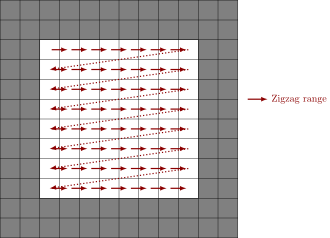
\includegraphics[width=0.8\textwidth]{../figures/linear_rng}
      \caption{Range-v3's ranges}
    \end{figure}

    \column{0.50\textwidth}
    \begin{figure}
      \includegraphics[width=0.8\textwidth]{../figures/segmented_rng}
      \caption{Segmented ranges}
    \end{figure}
  \end{columns}
\end{frame}

\begin{frame}[fragile]{Efficient way to traverse an image}
  Compiler needs explicit contiguous dimension to generate vectorized instructions.
  \begin{columns}[T,onlytextwidth]
    \column{0.50\textwidth}
    Milena's algorithm (unvectorized):
    \begin{minted}{C++}
template <class I, class O, class SE>
void dilate(const Image<I>& input_, Image<O>& output_, const SE& se)
{
    const I& input = exact(input_);
    O& output = exact(output_);
    mln_piter(I)  p(input.domain());
    mln_qiter(SE) n(se, p);
    for_all(p)
    {
        mln_value(I) M = f(p);
        for_all(q)
            M = max(f(q), M);
        output(p) = M;
    }
}
    \end{minted}
    \column{0.50\textwidth}

  \end{columns}
\end{frame}

\begin{frame}[fragile]{Efficient way to traverse an image}
  Compiler needs explicit contiguous dimension to generate vectorized instructions.
  \begin{columns}[T,onlytextwidth]
    \column{0.50\textwidth}
    Pylene's v1, unoptimized algorithm:
    \begin{minted}{C++}
template<Image I, OutputImage O, class SE>
  requires (StructuringElement<SE,
              image_point_t<I>>)
void dilate(I input, O output, SE se) {
    mln_foreach(auto p, input.domain()) {
        auto M = input(p);
        for(auto n : se(p))
            M = std::max(M, f(n));
        output(p) = M;
    }
}
    \end{minted}
    \column{0.50\textwidth}
    Pylene's v2, optimized algorithm using pixels (segmented ranges under the hood):
    \begin{minted}{C++}
template<Image I, OutputImage O, class SE>
  requires (StructuringElement<SE,
              image_point_t<I>>)
void dilate(I input, O output, SE se) {
    auto z = view::zip(input.pixels(),
                output.pixels());
    mln_foreach((auto [pxin, pxout]), z) {
        auto M = pxin.val();
        for(auto nx : se(pxin))
            M = std::max(M, nx.val());
        pxout.val() = M;
    }
}
    \end{minted}
  \end{columns}
\end{frame}


\begin{frame}[fragile]{Concept formal definition}
  \small
  \begin{table}[htbp]
    \begin{scriptsize}
      \begin{tabular}{l|l|l|l|}
        \cline{2-4}
                                                     & \thead{Definition }               &
        \thead{Description}                          & \thead{Requirement}                                      \\
        % Image
        \cline{1-4}
        \multicolumn{1}{|c|}{\multirow{3}{*}{Image}} & \texttt{Ima::const\_pixel\_range} & \makecell[l]{type of
          the range to iterate over
        \\ all the constant pixels} & \makecell[l]{models the concept \\
          \emph{ForwardRange}}
        \\
        \cline{2-4}
        \multicolumn{1}{|c|}{}                       & \texttt{Ima::pixel\_type}         & type of a pixel
                                                     & models the concept \emph{Pixel}                          \\
        \cline{2-4}
        \multicolumn{1}{|c|}{}                       & \texttt{Ima::value\_type}         & type of a value
                                                     & models the concept \emph{Regular}                        \\
        \cline{1-4}
        % Writable Image
        \multicolumn{1}{|c|}{\makecell[l]{Writable
        \\ Image}} & \texttt{WIma::pixel\_range} & \makecell[l]{type of the range to iterate over
        \\ all the non-constant pixels} & \makecell[l]{models the concept \\
          \emph{ForwardRange}}
        \\
        \cline{1-4}
        % StructuringElement \multicolumn{1}{|c|}{StructuringElement} &  &  & \\
        %  \cline{1-4} Decomposable \multicolumn{1}{|c|}{Decomposable} &  &  & \\
        %  \cline{1-4}
      \end{tabular}
    \end{scriptsize}
    \caption{Concepts formalization: definitions}
    \label{table:concept.definitions}
  \end{table}
  \begin{table}[htbp]
    \begin{scriptsize}
      \begin{tabular}{l|l|l|l|}
        \cline{2-4}
                                          & \thead{Expression}                              & \thead{Return Type} &
        \thead{Description}                                                                                         \\
        \cline{1-4}
        % Image
        \multicolumn{1}{|c|}{Image}       & \texttt{cima.pixels()}                          &
        \texttt{Ima::const\_pixel\_range} & \makecell[l]{returns a range of constant pixels
        \\ to iterate over it} \\
        \cline{1-4}
        % Writable Image
        \multicolumn{1}{|c|}{\makecell[l]{Writable
        \\ Image}} &\texttt{wima.pixels()} & \texttt{WIma::pixel\_range}       & \makecell[l]{returns a range of
        pixels                                                                                                      \\ to iterate over it} \\
        \cline{1-4}
      \end{tabular}
    \end{scriptsize}
    \caption{Concepts formalization: expressions}
    \label{table:concept.expressions}
  \end{table}
\end{frame}

\begin{frame}[fragile]{Pylene's views vs. Milena's morphers vs. STL ranges' views}
  \begin{alertblock}{Differences with STL ranges' views}
    \begin{itemize}
      \item STL's views are distinct from STL's containers and are constructed from ranges.
      \item Ranges are constructed from a container (and their iterators)
      \item Views is 3 levels of abstraction above a container.
    \end{itemize}
  \end{alertblock}
  \begin{alertblock}{Differences with Milena's morphers}
    \begin{itemize}
      \item Milena's morphers were not cheap to copy.
      \item Constructed from an image's reference otherwise need of deep-copy.
      \item As base image was taken by reference, possibility of dangling pointers.
      \item Dangle happens when chaining transformations with pipe (temporary copies).
      \item Const semantic (const values vs. writable values) ill-defined.
    \end{itemize}
  \end{alertblock}
\end{frame}

\begin{frame}{Static-dynamic bridge: languages type}
  \begin{figure}[htbp]
    \centering
    \includegraphics[width=.75\textwidth]{../figures/comp_inter_hybrid_summary}
    \caption{Languages types: summary diagram}
  \end{figure}
\end{frame}

\begin{frame}{Static information vs. dynamic information}
  \begin{alertblock}{Static information (known at compile-time)}
    \begin{itemize}
      \item Image's value type (unit8, rgb8, complex, etc.),
      \item Image's dimension size (1D, 2D, 3D, etc.),
      \item Architecture of the hardware hosting the program (x86, ARM, PowerPC, GPU, etc.).
    \end{itemize}
  \end{alertblock}
  \begin{alertblock}{Dynamic information (known at runtime)}
    \begin{itemize}
      \item Image's actual values,
      \item Image's actual size,
      \item Architecture of the hardware hosting the program (x86, ARM, PowerPC, GPU, etc.).
    \end{itemize}
  \end{alertblock}
\end{frame}

\end{document}